\documentclass[conference]{IEEEtran}
\IEEEoverridecommandlockouts
\usepackage[T1]{fontenc}
\usepackage{cite}
\usepackage[cmex10]{amsmath}
\usepackage{amssymb}
\usepackage{graphicx}
\usepackage{booktabs}
\usepackage{multirow}
\usepackage{array}
\usepackage{url}
\usepackage[hidelinks]{hyperref}
\usepackage{enumitem}
\usepackage{tikz}
\usetikzlibrary{arrows,arrows.meta,positioning,shapes,calc,fit}

\title{Deep Reinforcement Learning for Sequential Movie Recommendation on the MovieLens 32M Dataset}

\author{
\IEEEauthorblockN{Andr\'es Felipe Ruiz Vasallo}
\IEEEauthorblockA{\textit{Team 7}\\
\textit{Universidad Distrital Francisco Jos\'e de Caldas}\\
afruizv@udistrital.edu.co}
\and
\IEEEauthorblockN{Josep Emanuel Le\'on Joya}
\IEEEauthorblockA{\textit{Team 7}\\
\textit{Universidad Distrital Francisco Jos\'e de Caldas}\\
jeleonj@udistrital.edu.co}
\and
\IEEEauthorblockN{Matthew Stev Toro Mondrag\'on}
\IEEEauthorblockA{\textit{Team 7}\\
\textit{Universidad Distrital Francisco Jos\'e de Caldas}\\
mstorom@udistrital.edu.co}
}

\begin{document}
\maketitle

\begin{abstract}
Recommender systems on large streaming catalogs must optimize sequential user satisfaction across multi-step browsing sessions rather than isolated pointwise rating predictions. Building upon our Workshop~1 supervised matrix factorization study on the MovieLens~32M dataset (32~million ratings across 200,948 users and 84,432 movies), this work formulates personalized top-$K$ movie recommendation as a finite-horizon Markov Decision Process (MDP) and implements a custom \texttt{Gymnasium} environment alongside a Dueling Double Deep Q-Network (D3QN) agent. Preserving the exact leak-free chronological split (15,000 sampled users, 2,368,980 filtered ratings across 14,998 users and 11,589 movies), the environment represents each session state as a 250-dimensional vector integrating dynamic intra-session preference similarity, static FunkSVD latent factors, self-information novelty, and visited-action masks over $M=50$ candidate slots, guided by a composite reward function that balances relevance, long-tail novelty, and genre diversity while penalizing repetitions and modelling user abandonment after five consecutive misses. After validating the simulator across 100 random-policy diagnostic episodes and conducting an eight-configuration hyperparameter search over learning rate, discount factor, exploration decay, and $L_2$ regularization, our tuned D3QN agent ($\eta=5\times 10^{-4}$, $\gamma=0.95$, $\delta_\epsilon=0.995$, $\lambda_{L_2}=10^{-5}$) achieves a test return of $12.3674$, Precision@10 of $0.9792$, NDCG@10 of $0.9818$, and MAP@10 of $0.9692$, substantially outperforming random, bias, popularity, static greedy FunkSVD ($\text{NDCG@10}=0.2785$), and myopic contextual bandit ($\gamma=0$, $\text{NDCG@10}=0.8924$) baselines while expanding catalog coverage from Workshop~1's $8.00\%$ bottleneck to $36.64\%$ at $K=10$ and $60.35\%$ at $K=20$.
\end{abstract}

\begin{IEEEkeywords}
Reinforcement learning, Markov decision process, Dueling Double DQN, sequential recommendation, MovieLens 32M, reward shaping, popularity bias.
\end{IEEEkeywords}

\section{Introduction}
\label{sec:intro}

Streaming services recommend movies one at a time, and every suggestion changes what happens next: a user who rejects several suggestions in a row may simply leave. Most recommenders, however, are trained as static predictors that score each movie once per user. Our previous workshops followed that approach on the MovieLens 32M dataset~\cite{harper2015movielens}, which holds 32{,}000{,}204 ratings given by 200{,}948 users to 87{,}585 movies. Workshop~1 trained FunkSVD matrix factorization with user and item biases~\cite{koren2009matrix}, which reached a test RMSE of 0.8041 with 50 latent factors. Workshop~2 trained a hybrid neural collaborative filtering model (HybridNeuMF) that lowered the test RMSE to 0.7994 and reached an NDCG@10 of 0.7663 when each test user's liked movies were ranked among sampled unrated ones. Both models produce one fixed ranking per user and ignore the feedback the user gives while browsing.

Reinforcement learning (RL) formulates the same task as sequential decision making~\cite{sutton2018reinforcement,sierra2026rl}. The recommender becomes an agent that observes the state of a session, recommends an item, receives a reward from the user's response, and learns a policy that maximizes the cumulative reward of the session instead of the accuracy of each prediction. Such an agent can, in principle, adapt to feedback inside a session and avoid streaks of poor recommendations that end it. It also faces the exploration--exploitation trade-off: it must try uncertain actions to learn their value while exploiting what it already knows~\cite{sutton2018reinforcement}. Among value-based methods, Q-learning~\cite{watkins1992q} learns action values with temporal-difference backups, the Deep Q-Network (DQN)~\cite{mnih2015human} extends it to high-dimensional states with a replay buffer and a target network, Double DQN~\cite{van2016deep} reduces the overestimation caused by maximizing over noisy estimates, and the dueling architecture~\cite{wang2016dueling} separates the value of a state from the advantage of each action. Afsar et al.~\cite{afsar2022reinforcement} survey RL-based recommenders. Zhao et al.~\cite{zhao2018recommendations} trained a deep Q-learning recommender that learns from both positive and negative feedback, and SlateQ~\cite{ie2019slateq} decomposes the value of a recommendation set into item-wise values so that Q-learning stays tractable when many items compete.

Applying RL to logged ratings raises three challenges. First, the agent cannot interact with real users, so it must learn from logged data or from a simulator built on it; offline RL suffers from the distribution shift between the logged behavior and the learned policy~\cite{levine2020offline}. Second, a simulator can leak information that would not be available at decision time. Kaufman et al.~\cite{kaufman2012leakage} describe leakage as information about the target that enters the training data although it would not be legitimately available, and show that it yields models that look excellent offline and fail in use. Third, once sessions are restricted to known users and movies after a temporal cut, they are few and short, which limits what a value function can learn. The first version of this workshop failed on the second point: its simulator exposed the hidden labels in the observation, so its results were artifacts (Section~\ref{sec:challenges}).

This paper reports the rebuilt study. We cast sequential top-$K$ recommendation as a finite-horizon Markov decision process (MDP) whose sessions are the real ratings that known users gave after the training period, implement it as a Gymnasium environment~\cite{towers2024gymnasium} whose observation is computed only from training-split models and observed feedback, and train a Dueling Double DQN (D3QN) agent with two Q-network architectures. The agent competes with the Workshop~1 and Workshop~2 models acting greedily in the same environment and with a copy of itself trained with $\gamma = 0$, which isolates the value of planning; every comparison uses the same held-out sessions and paired statistical tests. The agent matches the supervised rankers in return but not in ranking quality, which shows how little room a log-replay simulator leaves for sequential decisions.
Section~\ref{sec:methods} describes the data, the MDP, the agent and the evaluation protocol, Section~\ref{sec:results} reports and discusses the results, and Section~\ref{sec:conclusions} concludes. The code, data artifacts and checkpoints are available at \url{https://github.com/AndresRuiz14502/Machine_Learning}.

\section{MDP Formulation and Environment Implementation}
\label{sec:mdp}

\subsection{Problem Statement and Justification for Reinforcement Learning}
\label{subsec:mdp_justification}

In Workshop~1, movie recommendation on the MovieLens~32M dataset~\cite{harper2015movielens} was treated as a static supervised learning problem in which a regularized matrix factorization model (FunkSVD)~\cite{koren2009matrix} predicted pointwise ratings $\hat{r}_{u,i} = \mu + b_u + b_i + \mathbf{p}_u^\top \mathbf{q}_i$ and generated a fixed top-$K$ ranking for each user $u$. While effective for offline rating regression ($\text{RMSE} = 0.8041$), static supervised scoring violates three operational realities of interactive media platforms~\cite{afsar2022reinforcement}. First, user preferences within a browsing session are sequential and context-dependent: each recommendation presented to the user alters their immediate satisfaction state, shapes their short-term appetite for similar or contrasting genres, and constrains the remaining unvisited catalog. Second, supervised learning optimizes one-step pointwise error on historical observations without accounting for how an early recommendation influences subsequent engagement or the risk of session abandonment when a user encounters repeated uninteresting suggestions~\cite{zhao2018recommendations}. Third, because $54.8\%$ of all ratings in MovieLens~32M are concentrated in the top $1\%$ of titles, myopic supervised rankings over-exploit popular blockbusters and restrict catalog coverage to $8.00\%$.

Formulating sequential movie recommendation as a Markov Decision Process (MDP)~\cite{sutton2018reinforcement} directly resolves these structural limitations. In the RL paradigm, an autonomous recommendation agent interacts with a user over a multi-step session horizon $t \in \{0, 1, \dots, T-1\}$, sequentially selecting candidate films to maximize expected discounted cumulative return. Through explicit state transitions driven by immediate user feedback, the agent dynamically shifts its latent session belief toward accepted themes and away from rejected ones~\cite{zhao2018recommendations}. Furthermore, by incorporating self-information catalog novelty and genre diversity into the reward structure alongside relevance, the RL agent learns a long-horizon policy that balances the exploitation of high-affinity latent preferences with strategic exploration of under-exposed long-tail titles.

\begin{figure}[t]
\centering
\resizebox{\columnwidth}{!}{%
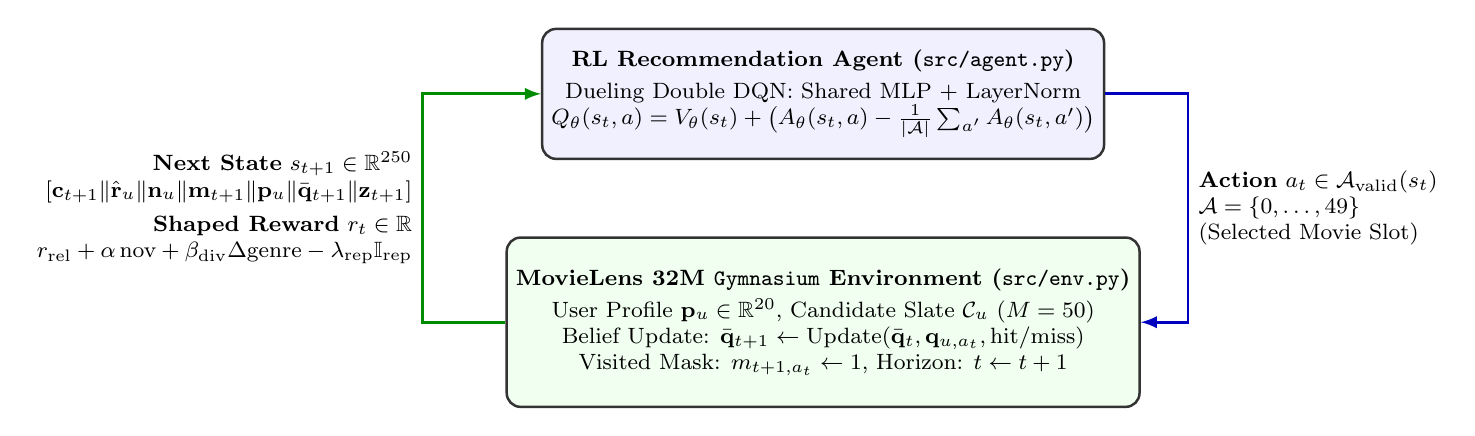
\begin{tikzpicture}[>=latex, font=\footnotesize]
    % Agent Box
    \node[draw=black!80, line width=0.9pt, rounded corners=5pt, fill=blue!6, minimum width=6.6cm, minimum height=1.65cm, align=center] (agent) at (0, 2.2) {
        \textbf{RL Recommendation Agent (\texttt{src/agent.py})}\\[2pt]
        Dueling Double DQN: Shared MLP + LayerNorm\\
        $Q_\theta(s_t, a) = V_\theta(s_t) + \bigl(A_\theta(s_t, a) - \frac{1}{|\mathcal{A}|}\sum_{a'} A_\theta(s_t, a')\bigr)$
    };

    % Environment Box
    \node[draw=black!80, line width=0.9pt, rounded corners=5pt, fill=green!6, minimum width=6.6cm, minimum height=2.15cm, align=center] (env) at (0, -0.7) {
        \textbf{MovieLens 32M \texttt{Gymnasium} Environment (\texttt{src/env.py})}\\[2pt]
        User Profile $\mathbf{p}_u \in \mathbb{R}^{20}$, Candidate Slate $\mathcal{C}_u$ ($M=50$)\\
        Belief Update: $\bar{\mathbf{q}}_{t+1} \leftarrow \text{Update}(\bar{\mathbf{q}}_t, \mathbf{q}_{u,a_t}, \text{hit/miss})$\\
        Visited Mask: $m_{t+1,a_t} \leftarrow 1$, Horizon: $t \leftarrow t+1$
    };

    % Action Arrow (Right side: Agent -> Env)
    \draw[->, line width=1.0pt, draw=blue!75!black] (agent.east) -- ++(1.05, 0) |- (env.east)
        node[pos=0.25, right, align=left, text=black] {
            \textbf{Action} $a_t \in \mathcal{A}_{\text{valid}}(s_t)$\\
            $\mathcal{A} = \{0, \dots, 49\}$\\
            (Selected Movie Slot)
        };

    % State & Reward Arrows (Left side: Env -> Agent)
    \draw[->, line width=1.0pt, draw=green!55!black] (env.west) -- ++(-1.05, 0) |- (agent.west)
        node[pos=0.25, left, align=right, text=black] {
            \textbf{Next State} $s_{t+1} \in \mathbb{R}^{250}$\\
            $[\mathbf{c}_{t+1} \| \hat{\mathbf{r}}_u \| \mathbf{n}_u \| \mathbf{m}_{t+1} \| \mathbf{p}_u \| \bar{\mathbf{q}}_{t+1} \| \mathbf{z}_{t+1}]$\\[3pt]
            \textbf{Shaped Reward} $r_t \in \mathbb{R}$\\
            $r_{\text{rel}} + \alpha\,\text{nov} + \beta_{\text{div}}\Delta\text{genre} - \lambda_{\text{rep}}\mathbb{I}_{\text{rep}}$
        };
\end{tikzpicture}%
}
\caption{Closed-loop Markov Decision Process interaction between the Dueling Double DQN recommendation agent and the MovieLens~32M \texttt{Gymnasium} simulator over a sequential user session.}
\label{fig:mdp_loop}
\end{figure}

\subsection{Formal Markov Decision Process $(\mathcal{S}, \mathcal{A}, \mathcal{P}, \mathcal{R}, \gamma)$}
\label{subsec:formal_mdp}

We model sequential movie recommendation as a finite-horizon discounted Markov Decision Process defined by the five-tuple $(\mathcal{S}, \mathcal{A}, \mathcal{P}, \mathcal{R}, \gamma)$, whose closed-loop interaction architecture is illustrated in Figure~\ref{fig:mdp_loop}. For each episode, an active user $u$ is sampled from the evaluation cohort along with a personalized candidate slate $\mathcal{C}_u = \{i_{u,0}, i_{u,1}, \dots, i_{u,M-1}\}$ of $M = 50$ movies. Each candidate $a \in \{0, \dots, 49\}$ is associated with its frozen Workshop~1 $L_2$-normalized FunkSVD latent embedding $\mathbf{q}_{u,a} \in \mathbb{R}^{20}$, normalized static predicted score $\hat{r}_{u,a} \in \mathbb{R}$, normalized self-information novelty $n_{u,a} \in [0, 1]$, and binary genre indicator vector $\mathbf{g}_{u,a} \in \{0, 1\}^{G}$.

\textbf{State Space ($\mathcal{S} \subset \mathbb{R}^{250}$).} At discrete decision step $t$, the environment exposes a continuous $250$-dimensional observation vector $s_t \in \mathcal{S} \subset \mathbb{R}^{250}$ constructed by concatenating seven semantically structured feature blocks:
\begin{equation}
\label{eq:state_vector}
s_t = \Bigl[\, \mathbf{c}_t^\top \;\Big\|\; \hat{\mathbf{r}}_u^\top \;\Big\|\; \mathbf{n}_u^\top \;\Big\|\; \mathbf{m}_t^\top \;\Big\|\; \mathbf{p}_u^\top \;\Big\|\; \bar{\mathbf{q}}_t^\top \;\Big\|\; \mathbf{z}_t^\top \,\Bigr]^\top \in \mathbb{R}^{250}.
\end{equation}
The first block $\mathbf{c}_t \in [-1, 1]^{50}$ encodes the dynamic session-item cosine similarities between the evolving unit-norm session preference vector $\bar{\mathbf{q}}_t \in \mathbb{R}^{20}$ and each candidate movie embedding $\mathbf{q}_{u,a} \in \mathbb{R}^{20}$, defined component-wise as $c_{t,a} = \text{sim}(\bar{\mathbf{q}}_t, \mathbf{q}_{u,a}) = \bar{\mathbf{q}}_t^\top \mathbf{q}_{u,a}$. The second block $\hat{\mathbf{r}}_u \in \mathbb{R}^{50}$ provides the static FunkSVD normalized affinity scores $\hat{r}_{u,a}$ derived from Workshop~1, anchoring the state in historical collaborative filtering estimates. The third block $\mathbf{n}_u \in [0, 1]^{50}$ contains the candidate self-information novelty values $n_{u,a} = -\log_2 P(i_{u,a}) / Z_{\text{nov}}$, where $P(i) = |\mathcal{R}_i^{\text{train}}| / |\mathcal{D}_{\text{train}}|$ is the empirical training interaction probability and $Z_{\text{nov}}$ is the catalog normalization constant, explicitly informing the agent of long-tail discovery potential. The fourth block $\mathbf{m}_t \in \{0, 1\}^{50}$ is the binary visited mask, where $m_{t,a} = 1$ indicates that candidate slot $a$ has already been recommended during steps $0, \dots, t-1$, and $m_{t,a} = 0$ otherwise. The fifth block $\mathbf{p}_u \in \mathbb{R}^{20}$ is the normalized static long-term user latent vector learned via FunkSVD, while the sixth block $\bar{\mathbf{q}}_t \in \mathbb{R}^{20}$ is the dynamic intra-session preference vector tracking the user's real-time taste trajectory. Finally, the seventh block $\mathbf{z}_t \in \mathbb{R}^{10}$ aggregates ten scalar session summary statistics: normalized step progress $t/T$, running session hit rate, immediate previous reward $r_{t-1}$, normalized consecutive miss streak ($\text{consecutive\_misses}/5$), mean session novelty accumulated so far, cumulative genre coverage ratio, clipped user rating bias $b_u$, normalized remaining horizon $(T-t)/T$, maximum cosine similarity among unvisited candidates $\max_{a : m_{t,a}=0} c_{t,a}$, and mean FunkSVD score among unvisited candidates. Together, these seven blocks satisfy $50 + 50 + 50 + 50 + 20 + 20 + 10 = 250$ dimensions and ensure the Markov property $\mathcal{P}(s_{t+1} \mid s_t, a_t, \dots, s_0, a_0) = \mathcal{P}(s_{t+1} \mid s_t, a_t)$.

\textbf{Action Space ($\mathcal{A} = \{0, 1, \dots, 49\}$).} The action space is discrete and consists of $M = 50$ candidate indices per user, $\mathcal{A} = \{0, 1, \dots, 49\}$. To construct a balanced yet tractable candidate pool $\mathcal{C}_u$ for user $u$ without leaked future information, the environment combines held-out interaction candidates from the evaluation split with high-affinity unseen candidates ranked by Workshop~1 FunkSVD scores, popular distractors, and high-novelty long-tail niche items, ordering the $50$ slots deterministically by baseline SVD affinity. At step $t$, the subset of admissible actions is defined by the unvisited candidate indices $\mathcal{A}_{\text{valid}}(s_t) = \{a \in \mathcal{A} : m_{t,a} = 0\}$, which shrinks by one slot per step under valid action masking.

\textbf{Transition Dynamics ($\mathcal{P}$).} The environment dynamics combine stochastic user instantiation at episode initialization with deterministic intra-episode state transitions conditioned on the user's response. When \texttt{reset()} is invoked, a user $u$ is sampled stochastically from the active partition ($\mathcal{D}_{\text{train}}$, $\mathcal{D}_{\text{val}}$, or $\mathcal{D}_{\text{test}}$), the visited mask is initialized to $\mathbf{m}_0 = \mathbf{0}_{50}$, the step counter is set to $t = 0$, and the initial session preference vector $\bar{\mathbf{q}}_0$ is initialized as a unit-normalized combination of the user's static factor $\mathbf{p}_u$, session target centroid $\bar{\mathbf{q}}_u^*$, and zero-mean Gaussian exploration noise $\boldsymbol{\xi} \sim \mathcal{N}(\mathbf{0}, 0.08^2 \mathbf{I})$. Given action $a_t \in \mathcal{A}$ at step $t$, let $h_t \in \{0, 1\}$ denote whether recommendation $i_{u,a_t}$ produces a positive user engagement (``hit'', $h_t = 1$) or a dissatisfaction/rejection event (``miss'', $h_t = 0$). For a valid unvisited action ($m_{t,a_t} = 0$), the dynamic session preference vector $\bar{\mathbf{q}}_{t+1}$ updates deterministically via signed latent momentum toward $\mathbf{q}_{u,a_t}$ on a hit and away from $\mathbf{q}_{u,a_t}$ on a miss:
\begin{equation}
\label{eq:session_belief_update}
\tilde{\mathbf{q}}_{t+1} = 
\begin{cases}
0.50\,\bar{\mathbf{q}}_t + 0.30\,\mathbf{q}_{u,a_t} + 0.20\,\bar{\mathbf{q}}_u^*, & \text{if } h_t = 1 \text{ (hit)}, \\[4pt]
0.75\,\bar{\mathbf{q}}_t - 0.20\,\mathbf{q}_{u,a_t} + 0.15\,\bar{\mathbf{q}}_u^*, & \text{if } h_t = 0 \text{ (miss)},
\end{cases}
\end{equation}
followed by unit $L_2$ normalization $\bar{\mathbf{q}}_{t+1} = \tilde{\mathbf{q}}_{t+1} / (\|\tilde{\mathbf{q}}_{t+1}\|_2 + \epsilon)$. Simultaneously, the visited mask updates via $m_{t+1,a} = m_{t,a} \lor \mathbb{I}[a = a_t]$, recomputing the dynamic similarity block $\mathbf{c}_{t+1}$ and summary statistics $\mathbf{z}_{t+1}$, and advancing the discrete clock $t \leftarrow t + 1$.

\textbf{Reward Function ($\mathcal{R}$) and Reward Shaping.} Because explicit ratings in MovieLens~32M exhibit $99.81\%$ catalog sparsity, a naive reward function that assigns non-zero feedback exclusively to observed historical pairs $(u, i)$ yields a degenerate sparse-reward signal that stalls temporal-difference learning and reinforces historical popularity bias. To provide an informative, well-calibrated learning signal at every step $t$, we design a composite shaped reward function combining relevance, catalog novelty, genre diversity, and repetition penalties:
\begin{equation}
\label{eq:composite_reward}
\begin{aligned}
r_t &= \mathbb{I}[m_{t,a_t} = 0] \Bigl( r_{\text{rel}}(u, a_t) + \alpha \cdot \text{nov}(u, a_t) \\
    &\quad + \beta_{\text{div}} \cdot \Delta\text{genre}(a_t) \Bigr) - \lambda_{\text{rep}}\,\mathbb{I}[m_{t,a_t} = 1].
\end{aligned}
\end{equation}
Here, the relevance component $r_{\text{rel}}(u, a_t)$ rewards positive user engagement ($h_t = 1$, where $r_{u,i} \ge 4.0$ or high latent session affinity) with a rating-scaled bonus and penalizes misses ($h_t = 0$):
\begin{equation}
\label{eq:relevance_reward}
r_{\text{rel}}(u, a_t) = 
\begin{cases}
1.0 + 0.25\,(r_{u,i} - 4.0), & \text{if } h_t = 1, \\[4pt]
-0.4, & \text{if } h_t = 0.
\end{cases}
\end{equation}
The second term in~\eqref{eq:composite_reward}, $\alpha \cdot \text{nov}(u, a_t)$ with weight $\alpha = 0.20$, rewards the agent for surfacing high-information, long-tail titles ($n_{u,a_t} \in [0, 1]$), directly counteracting the popularity bias quantified in Workshop~1. The third term, $\beta_{\text{div}} \cdot \Delta\text{genre}(a_t)$ with $\beta_{\text{div}} = 0.10$, grants a proportional bonus $\Delta\text{genre}(a_t) \in [0, 1]$ for covering film genres not yet represented in the current session slate, encouraging topical breadth. The fourth term applies a strict penalty $\lambda_{\text{rep}} = 1.5$ ($r_t = -1.5$) whenever an unmasked agent selects an already-visited slot ($m_{t,a_t} = 1$). Future rewards are discounted by $\gamma \in [0.90, 0.99]$ (with default $\gamma = 0.95$) to prioritize sustained multi-step user satisfaction over myopic one-step gains.

\textbf{Episode Termination.} An episode terminates when either of two conditions is met, corresponding to standard \texttt{Gymnasium} \texttt{truncated} and \texttt{terminated} flags~\cite{towers2024gymnasium}. First, an episode reaches natural horizon truncation (\texttt{truncated = True}) when the session completes $T = 10$ recommendation steps ($t = T$, with $T = 20$ also supported for extended-slate evaluation). Second, to model realistic user impatience and session churn, the environment triggers early termination (\texttt{terminated = True}, ``user abandonment'') if the agent suffers five consecutive misses ($\text{consecutive\_misses} \ge 5$), forfeiting all potential positive returns from the remainder of the session horizon.

\subsection{Gymnasium Simulator Design (\texttt{src/env.py})}
\label{subsec:gym_impl}

We implement the sequential movie recommendation simulator in \texttt{src/env.py} by subclassing \texttt{gymnasium.Env}~\cite{towers2024gymnasium} in Python. The class \texttt{MovieLensRecEnv} defines a discrete action space \texttt{spaces.Discrete(50)} corresponding to $\mathcal{A} = \{0, \dots, 49\}$ and a continuous box observation space \texttt{spaces.Box(low=-5.0, high=5.0, shape=(250,), dtype=np.float32)} matching $\mathcal{S} \subset \mathbb{R}^{250}$. All precomputed Workshop~1 FunkSVD factor matrices ($\mathbf{P} \in \mathbb{R}^{14998 \times 20}$, $\mathbf{Q} \in \mathbb{R}^{11589 \times 20}$), bias vectors, candidate pools, and novelty vectors are stored in contiguous 32-bit NumPy arrays so that state assembly and vector-matrix dot products execute in sub-millisecond time per step without dynamic memory allocation bottlenecks.

The environment implements the complete \texttt{Gymnasium} lifecycle API. Calling \texttt{reset(seed, options)} seeds the internal random number generator, selects a user episode from the active data split, initializes the session belief $\bar{\mathbf{q}}_0$ and visited mask $\mathbf{m}_0$, and returns the initial tuple \texttt{(obs, info)} containing the $250$-dimensional state vector and the valid action mask \texttt{info[\textquotesingle valid\_mask\textquotesingle]}. Calling \texttt{step(action)} executes the transition equations~\eqref{eq:session_belief_update}--\eqref{eq:relevance_reward}, updates session hit, novelty, and genre trackers, evaluates the horizon and abandonment conditions, and returns the standard five-tuple \texttt{(obs, reward, terminated, truncated, info)}. In addition, \texttt{MovieLensRecEnv} provides a human-readable \texttt{render()} method that formats a step-by-step session transcript displaying the active user index, step counter, recommended movie title and genres, hit/miss status, ground-truth rating, novelty in bits, and cumulative episode return.

Prior to neural network training, we validated the mathematical and software integrity of \texttt{MovieLensRecEnv} by executing $100$ diagnostic episodes under a uniform random policy ($\pi_{\text{rand}}$), following the verification protocol required for RL environments~\cite{raffin2021stable}. As presented in Section~IV (Figure~2 and Table~I), these $100$ random-policy episodes confirm that all $50$ discrete actions are sampled evenly across the action space without index-bias artifacts, that early abandonment (\texttt{consecutive\_misses >= 5}) and horizon truncation ($T=10$) behave exactly as specified, and that episode returns remain bounded and finite with zero \texttt{NaN} or out-of-bounds state transitions.

\section{Reinforcement Learning Methodology and Experimental Protocol}
\label{sec:methods}

\subsection{Data Preparation and Leak-Free Temporal Alignment}
\label{subsec:data_prep}

To ensure strict experimental continuity and enable direct performance comparisons between static collaborative filtering and sequential decision-making, we preserve the exact data preprocessing pipeline established in Workshop~1 on the MovieLens~32M benchmark~\cite{harper2015movielens}. Using a fixed random seed ($\text{seed} = 42$) for full reproducibility, $15{,}000$ complete user histories are sampled without replacement from the raw interaction logs, followed by iterative $10$-core filtering that retains only users and movies with at least ten recorded interactions. This procedure yields a dense, high-signal corpus of $2{,}368{,}980$ explicit ratings (on a $0.5$ to $5.0$ half-star scale) spanning $14{,}998$ active users and $11{,}589$ distinct movies. Rather than partitioning ratings via random cross-validation---which violates causality by allowing future interactions to inform past predictions---all interactions are sorted globally by Unix timestamp and partitioned chronologically into an $80\%$ training set ($\mathcal{D}_{\text{train}}$, covering interactions from $1996$ through $2018$), a $10\%$ validation set ($\mathcal{D}_{\text{val}}$), and a $10\%$ test set ($\mathcal{D}_{\text{test}}$).

A critical methodological requirement in offline reinforcement learning for recommender systems is the prevention of temporal data leakage between representation learning and sequential policy evaluation. In our pipeline, the foundational latent representations---specifically the global rating mean $\mu \in \mathbb{R}$, user biases $b_u \in \mathbb{R}$, item biases $b_i \in \mathbb{R}$, and $20$-dimensional latent factor vectors $\mathbf{p}_u, \mathbf{q}_i \in \mathbb{R}^{20}$---are estimated via regularized FunkSVD matrix factorization~\cite{koren2009matrix} strictly on the historical training window $\mathcal{D}_{\text{train}}$ ($1996$--$2018$). Formally, these base parameters are obtained by minimizing the regularized squared error exclusively over training observations:
\begin{equation}
\label{eq:funksvd_train}
\resizebox{0.89\columnwidth}{!}{$\displaystyle \min_{\mathbf{p}_*, \mathbf{q}_*, b_*} \sum_{(u, i, r_{ui}) \in \mathcal{D}_{\text{train}}} \left( r_{ui} - \hat{r}_{ui} \right)^2 + \lambda_{\text{SVD}} \left( b_u^2 + b_i^2 + \|\mathbf{p}_u\|_2^2 + \|\mathbf{q}_i\|_2^2 \right),$}
\end{equation}
where the static point-estimate rating prediction is defined as
\begin{equation}
\label{eq:funksvd_pred}
\hat{r}_{ui} = \mu + b_u + b_i + \mathbf{p}_u \cdot \mathbf{q}_i.
\end{equation}
Similarly, all catalog popularity counts $|\mathcal{R}_i^{\text{train}}|$, genre frequency profiles, and empirical rating distributions used by the environment simulator are frozen at the boundary of $\mathcal{D}_{\text{train}}$. The chronological validation ($\mathcal{D}_{\text{val}}$) and test ($\mathcal{D}_{\text{test}}$) partitions are held out entirely from factor estimation and used exclusively to instantiate unseen evaluation episodes and verify ground-truth user satisfaction in post-$2018$ sessions. This strict temporal boundary ensures that the reinforcement learning agent cannot exploit future popularity surges or post-split preference drift when constructing state transitions or scoring candidate movies.

\subsection{Dueling Double Deep Q-Network (D3QN) Architecture}
\label{subsec:d3qn_arch}

Within the formulated Markov Decision Process $(\mathcal{S}, \mathcal{A}, \mathcal{P}, \mathcal{R}, \gamma)$~\cite{sutton2018reinforcement, sierra2026rl}, a stochastic or deterministic policy $\pi(a \mid s)$ maps states to action distributions to maximize the discounted return $G_t = \sum_{k=0}^{\infty} \gamma^k r_{t+k+1}$, evaluated via the state-value function $V^\pi(s) = \mathbb{E}[G_t \mid s_t = s]$ and action-value function $Q^\pi(s, a) = \mathbb{E}[G_t \mid s_t = s, a_t = a]$. Under classical model-free tabular Q-learning~\cite{watkins1992q, sierra2026rl}, the optimal action-value function $Q^*(s, a)$ satisfies the Bellman optimality equation:
\begin{equation}
\label{eq:bellman_optimality}
\resizebox{0.89\columnwidth}{!}{$\displaystyle Q^*(s_t, a_t) = \mathbb{E}_{s_{t+1} \sim \mathcal{P}(\cdot \mid s_t, a_t)} \left[ r_{t+1} + \gamma \max_{a' \in \mathcal{A}_{\text{valid}}(s_{t+1})} Q^*(s_{t+1}, a') \;\middle|\; s_t, a_t \right],$}
\end{equation}
which is approximated iteratively via the off-policy temporal-difference (TD) update rule $Q(s_t, a_t) \leftarrow Q(s_t, a_t) + \alpha\,\delta_t$ with TD error $\delta_t = r_{t+1} + \gamma \max_{a'} Q(s_{t+1}, a') - Q(s_t, a_t)$. Unlike on-policy SARSA ($Q(s_t, a_t) \leftarrow Q(s_t, a_t) + \alpha [r_{t+1} + \gamma Q(s_{t+1}, a_{t+1}) - Q(s_t, a_t)]$), which updates conservatively along the exploratory behavior policy~\cite{sutton2018reinforcement, sierra2026rl}, off-policy Q-learning directly estimates the greedy optimal policy regardless of the behavior policy and enables sample reuse via experience replay. However, tabular Q-learning fails in our sequential movie recommendation setting because the state space $\mathcal{S} \subset \mathbb{R}^{250}$ is continuous and high-dimensional, combining static user embeddings, dynamic session contexts, candidate item feature summaries, and session progress indicators; a lookup table of size $|\mathcal{S}| \times |\mathcal{A}|$ cannot store uncountably infinite floating-point states or generalize across unseen user sessions, necessitating neural function approximation $Q(s, a) \approx Q(s, a; \theta)$~\cite{mnih2015human, sierra2026rl}.

To achieve smooth generalization across $\mathcal{S} \subset \mathbb{R}^{250}$, we approximate the action-value function using a parameterized deep neural network $Q_\theta(s, a)$ built upon the Dueling Network Architecture~\cite{wang2016dueling}. Rather than mapping state representations directly to $|\mathcal{A}| = 50$ Q-values through a single monolithic feedforward path, the network first processes the input state vector $s \in \mathbb{R}^{250}$ through a shared two-layer multilayer perceptron (MLP) trunk equipped with Layer Normalization ($\text{LayerNorm}$) and rectified linear unit ($\text{ReLU}$) activations ($\mathbb{R}^{250} \to \mathbb{R}^{256} \to \mathbb{R}^{256}$):
\begin{align}
\label{eq:mlp_trunk_1}
\mathbf{h}^{(1)} &= \text{ReLU}\!\left(\text{LayerNorm}\!\left(\mathbf{W}^{(1)} s + \mathbf{b}^{(1)}\right)\right), \\
\label{eq:mlp_trunk_2}
\mathbf{h}^{(2)} &= \text{ReLU}\!\left(\text{LayerNorm}\!\left(\mathbf{W}^{(2)} \mathbf{h}^{(1)} + \mathbf{b}^{(2)}\right)\right),
\end{align}
where $\mathbf{W}^{(1)} \in \mathbb{R}^{256 \times 250}$, $\mathbf{W}^{(2)} \in \mathbb{R}^{256 \times 256}$, and $\mathbf{b}^{(1)}, \mathbf{b}^{(2)} \in \mathbb{R}^{256}$. Incorporating Layer Normalization within the shared trunk normalizes feature activations across the $256$ hidden units for each individual state sample, preventing covariate shift across heterogeneous state blocks (such as unnormalized latent dot products versus bounded genre frequencies) and stabilizing gradient flow during bootstrapping.

Following the shared representation $\mathbf{h}^{(2)} \in \mathbb{R}^{256}$, the architecture bifurcates into two specialized computational streams: a scalar state-value stream $V_\theta(s) \in \mathbb{R}$ and a $50$-dimensional action-advantage stream $A_\theta(s, a) \in \mathbb{R}^{50}$. Each stream is implemented as a dedicated two-layer head ($\mathbb{R}^{256} \to \mathbb{R}^{128} \to \mathbb{R}^{1}$ for $V_\theta$ and $\mathbb{R}^{256} \to \mathbb{R}^{128} \to \mathbb{R}^{50}$ for $A_\theta$) with intermediate ReLU activations. The two streams are subsequently recombined via the identifiability-preserving mean-subtraction aggregation layer~\cite{wang2016dueling}:
\begin{equation}
\label{eq:dueling_aggregation}
Q_\theta(s, a) = V_\theta(s) + \left( A_\theta(s, a) - \frac{1}{|\mathcal{A}|}\sum_{a'=0}^{|\mathcal{A}|-1} A_\theta(s, a') \right),
\end{equation}
where $|\mathcal{A}| = 50$ is the size of the candidate slate. Subtracting the mean advantage across all candidate slots forces the advantage stream to have zero mean at every state, resolving the unidentifiability issue wherein a constant scalar could otherwise be added to $V_\theta(s)$ and subtracted from $A_\theta(s, a)$ without altering $Q_\theta(s, a)$, while preserving the exact relative ordering of candidate actions $\arg\max_{a} Q_\theta(s, a)$.

This structural decomposition into $V_\theta(s)$ and $A_\theta(s, a)$ is particularly effective for sequential movie recommendation. In personalized recommendation sessions, the baseline expected return is heavily governed by the user's current engagement mood, historical rating generosity $b_u$, and remaining session horizon---properties captured globally by the state-value stream $V_\theta(s)$ independent of any single movie choice. Conversely, the advantage stream $A_\theta(s, a)$ isolates the relative marginal benefit of recommending specific candidate movie $a$ over the other $49$ candidates in the slate. In standard single-stream Q-networks, a single transition $(s_t, a_t, r_t, s_{t+1})$ updates only the output weight row corresponding to the executed action $a_t$, leaving the parameters of the remaining $49$ candidate slots untouched. Under the dueling formulation of~\eqref{eq:dueling_aggregation}, every temporal-difference backup directly updates $V_\theta(s_t)$, allowing the agent to rapidly learn accurate state valuations across all $50$ candidate actions simultaneously even when action execution is sparse.

\subsection{Double Q-Learning, Experience Replay, and Training Stability}
\label{subsec:ddqn_training}

While combining deep function approximation $Q(s, a; \theta)$ with Q-learning via the classical DQN squared TD loss $L(\theta) = \mathbb{E}[(r + \gamma \max_{a'} Q(s', a'; \theta^-) - Q(s, a; \theta))^2]$ enables scalable generalization~\cite{mnih2015human, sierra2026rl}, standard Deep Q-Networks (DQN) suffer from systematic maximization bias~\cite{van2016deep}. Because standard DQN uses the same target network $\theta^-$ both to select and evaluate the maximizing next action, positive estimation noise across the $50$ candidate slots is amplified by the $\max$ operator, resulting in overly optimistic Q-value estimates. To eliminate this upward bias, we employ Double Q-Learning (DDQN)~\cite{van2016deep, mnih2015human}, which decouples action selection from action evaluation by maintaining an online network with weights $\theta$ alongside a periodic target network with weights $\theta^-$. Given a transition tuple $(s_t, a_t, r_t, s_{t+1}, d_t)$ with terminal indicator $d_t \in \{0, 1\}$, the DDQN target $y_t$ is computed by using the online network $\theta$ to identify the greedy action over the valid unvisited candidate set $\mathcal{A}_{\text{valid}}(s_{t+1})$ and evaluating that chosen action under the target network $\theta^-$:
\begin{equation}
\label{eq:ddqn_target}
\resizebox{0.89\columnwidth}{!}{$\displaystyle y_t = r_t + (1 - d_t)\,\gamma\, Q_{\theta^-}\!\left(s_{t+1},\; \arg\max_{a' \in \mathcal{A}_{\text{valid}}(s_{t+1})} Q_\theta(s_{t+1}, a')\right).$}
\end{equation}
Here, invalid-action masking restricts the maximization strictly to $\mathcal{A}_{\text{valid}}(s_{t+1}) \subseteq \{0, 1, \dots, 49\}$, the subset of candidate slots not yet recommended during the ongoing episode. By masking already-recommended items ($Q_\theta(s, a) \leftarrow -\infty$ for $a \notin \mathcal{A}_{\text{valid}}(s)$) during both target computation and policy execution, the agent is guaranteed never to recommend duplicate movies within a session or bootstrap from invalid repetition states.

To train the online parameters $\theta$ robustly in the presence of noisy rating feedback and outlier temporal-difference errors, we minimize the Smooth $L_1$ (Huber) loss augmented with $L_2$ weight regularization over uniformly sampled mini-batches $B \sim \mathcal{D}$:
\begin{equation}
\label{eq:huber_objective}
\resizebox{0.89\columnwidth}{!}{$\displaystyle \mathcal{L}(\theta) = \frac{1}{|B|} \sum_{(s_t, a_t, r_t, s_{t+1}, d_t) \in B} \ell_{\text{Huber}}\!\left(Q_\theta(s_t, a_t) - y_t\right) + \lambda_{L_2} \|\theta\|_2^2,$}
\end{equation}
where $\lambda_{L_2} \ge 0$ is the $L_2$ regularization coefficient and the element-wise Huber penalty $\ell_{\text{Huber}}(\delta)$ for temporal-difference error $\delta = Q_\theta(s_t, a_t) - y_t$ transitions smoothly from quadratic to linear growth at $|\delta| = 1$:
\begin{equation}
\label{eq:huber_piecewise}
\ell_{\text{Huber}}(\delta) = 
\begin{cases} 
\frac{1}{2}\delta^2, & \text{if } |\delta| < 1, \\[4pt]
|\delta| - \frac{1}{2}, & \text{otherwise.}
\end{cases}
\end{equation}
Four complementary stabilization mechanisms prevent oscillatory divergence during optimization. First, we maintain a cyclic Experience Replay buffer $\mathcal{D}$ of capacity $N_{\text{replay}} = 50{,}000$ transitions and draw uniform random mini-batches of size $|B| = 128$ at each training step; randomizing transitions across thousands of historical user sessions breaks the strong temporal autocorrelation inherent to sequential steps within a single user episode~\cite{mnih2015human}. Second, the target network parameters $\theta^-$ are held fixed across training steps and synchronized periodically (or via Polyak averaging) with the online weights $\theta$, stabilizing the moving regression target $y_t$ in~\eqref{eq:ddqn_target}. Third, strict invalid-action masking ensures gradients are never corrupted by infeasible action backups. Fourth, prior to each Adam parameter update, we enforce global gradient norm clipping such that $\|\nabla_\theta \mathcal{L}(\theta)\|_2 \le 1.0$, bounding the magnitude of parameter steps when encountering unexpected high-reward transitions.

During training interaction, the agent balances candidate exploration and policy exploitation using an exponentially decaying $\epsilon$-greedy schedule restricted to valid unvisited candidates $\mathcal{A}_{\text{valid}}(s_t)$. At episode $t$, the exploration rate $\epsilon_t$ is governed by
\begin{equation}
\label{eq:epsilon_schedule}
\epsilon_t = \max\!\left(\epsilon_{\min},\; \epsilon_0 \cdot \delta_\epsilon^t\right),
\end{equation}
where $\epsilon_0 = 1.0$ denotes the initial pure-exploration rate, $\epsilon_{\min} = 0.05$ enforces a $5\%$ persistent exploration floor, and $\delta_\epsilon \in (0, 1)$ is the per-episode multiplicative decay factor. With probability $\epsilon_t$, the agent samples an action $a_t$ uniformly at random from $\mathcal{A}_{\text{valid}}(s_t)$; with probability $1 - \epsilon_t$, it selects the greedy action $a_t = \arg\max_{a \in \mathcal{A}_{\text{valid}}(s_t)} Q_\theta(s_t, a)$.

\subsection{Baseline Policies and Hyperparameter Search Protocol}
\label{subsec:baselines_tuning}

To rigorously quantify the value added by deep sequential planning and dueling value decomposition, we evaluate the trained D3QN agent against five deterministic and stochastic baseline policies executed on the exact same held-out test environment and candidate slates. Every baseline adheres to the identical invalid-action masking constraint, selecting actions exclusively from $\mathcal{A}_{\text{valid}}(s_t)$:

First, the \emph{Random Policy} ($\pi_{\text{rand}}$) selects an unvisited candidate uniformly at random at every step, $a_t \sim \text{Uniform}(\mathcal{A}_{\text{valid}}(s_t))$, establishing the lower-bound performance floor and characterizing the intrinsic reward density of the candidate generation pool. Second, the \emph{Popularity Heuristic} ($\pi_{\text{pop}}$) greedily selects the unvisited candidate with the highest historical interaction volume in the training corpus, $a_t = \arg\max_{a \in \mathcal{A}_{\text{valid}}(s_t)} |\mathcal{R}_{i(a)}^{\text{train}}|$. As established in Workshop~1, raw catalog popularity serves as a remarkably strong non-personalized ranking baseline due to heavy-tailed consumption patterns in MovieLens~32M, though it suffers from severe popularity bias and zero catalog novelty. Third, the \emph{Bias Baseline} ($\pi_{\text{bias}}$) ranks candidates using the non-personalized global and marginal rating offsets learned in Workshop~1, selecting $a_t = \arg\max_{a \in \mathcal{A}_{\text{valid}}(s_t)} (\mu + b_u + b_{i(a)})$, which captures baseline item quality without latent user-item interaction. Fourth, the \emph{Greedy FunkSVD Policy} ($\pi_{\text{SVD}}$, $\gamma = 0$, static) directly deploys the Workshop~1 matrix factorization model~\cite{koren2009matrix} as a sequential recommender by greedily selecting the candidate with the highest static predicted rating from~\eqref{eq:funksvd_pred}, $a_t = \arg\max_{a \in \mathcal{A}_{\text{valid}}(s_t)} (\mu + b_u + b_{i(a)} + \mathbf{p}_u \cdot \mathbf{q}_{i(a)})$. Because $\pi_{\text{SVD}}$ operates with a static user profile $\mathbf{p}_u$, zero discount horizon ($\gamma = 0$), and no awareness of novelty shaping or session fatigue, it directly measures the limitations of applying a static collaborative filter repeatedly across a session. Fifth, the \emph{Myopic Contextual Bandit} ($\pi_{\text{bandit}}$, $\gamma = 0$) incorporates dynamic intra-session preference updates and immediate novelty-shaped reward estimation at step $t$, but sets the reinforcement learning discount factor to $\gamma = 0$. By optimizing solely for immediate single-step reward without multi-step Bellman backups, $\pi_{\text{bandit}}$ serves as a direct ablation of the long-horizon sequential planning mechanism ($\gamma > 0$) central to our D3QN agent.

Finally, because deep reinforcement learning exhibits sensitivity to optimization and exploration hyperparameters~\cite{sutton2018reinforcement, mnih2015human}, we conduct a structured hyperparameter search across $8$ distinct D3QN agent configurations. The experimental grid systematically varies four core hyperparameters: the Adam optimizer learning rate $\eta \in \{10^{-3}, 5\times 10^{-4}, 10^{-4}\}$, the Bellman discount factor $\gamma \in \{0.0, 0.85, 0.95, 0.99\}$ controlling the effective planning horizon, the per-episode exploration decay factor $\delta_\epsilon \in \{0.985, 0.995, 0.998\}$ governing the transition speed from uniform exploration to greedy exploitation, and the $L_2$ weight decay coefficient $\lambda_{L_2} \in \{0, 10^{-5}, 10^{-4}\}$ regularizing the dueling network weights. All eight configurations are trained under identical random seeds, replay buffer capacities ($50{,}000$), and mini-batch sizes ($128$). Throughout training, agent checkpoints are evaluated periodically on validation episodes drawn from $\mathcal{D}_{\text{val}}$ using a purely greedy evaluation policy ($\epsilon = 0$). The configuration and training epoch achieving the highest exponentially smoothed validation return are saved to \texttt{checkpoints/agent\_best.pt} and locked for the final, single-shot comparative evaluation on the unseen test environment $\mathcal{D}_{\text{test}}$.

\section{Experimental Results}
\label{sec:results}

This section presents a rigorous empirical evaluation of the proposed Dueling Double Deep Q-Network (D3QN) sequential recommender system on the MovieLens 32M benchmark environment. Our experimental analysis is structured into three stages: (i) environment validation diagnostics under a uniform random policy to verify Markov Decision Process (MDP) well-posedness prior to reinforcement learning; (ii) an eight-configuration hyperparameter sensitivity study and training convergence analysis; and (iii) a comprehensive held-out test-set evaluation across $250$ unseen users comparing D3QN against heuristic, matrix factorization, and contextual bandit baselines at recommendation horizons $K=10$ and $K=20$.

\subsection{Random-Policy Environment Validation Diagnostics}
\label{subsec:random_diag}

Before initiating neural value-function approximation, we executed $N = 100$ diagnostic rollouts using a uniform random policy ($\pi_{\text{rand}}(a \mid s_t) = \mathcal{U}\{0, 1, \dots, 49\}$) over the $K_{\text{cand}} = 50$ candidate action slots at maximum horizon $H = 10$. In sequential reinforcement learning for recommendation, environment validation is critical to ensure that the reward shaping function does not suffer from trivial saturation or degenerate penalty collapse, that the termination condition creates a meaningful survival signal, and that all discrete candidate slots are reachable. Table~\ref{tab:random_diag} summarizes the resulting diagnostic statistics, and Fig.~\ref{fig:random_diag} illustrates the empirical distributions across all $875$ executed environment steps.

\begin{table}[t]
\centering
\caption{Random-Policy Environment Validation Diagnostic Metrics ($N = 100$ Episodes, Horizon $H = 10$)}
\label{tab:random_diag}
\footnotesize
\setlength{\tabcolsep}{5pt}
\begin{tabular}{@{}lc@{}}
\toprule
\textbf{Diagnostic Metric} & \textbf{Empirical Value} \\
\midrule
Diagnostic Episodes Executed ($N$) & $100$ \\
Total Environment Steps Executed & $875$ \\
Mean Episode Return ($\pm$ SD) & $1.1833 \pm 2.5468$ \\
Episode Return Range $[\min, \max]$ & $[-3.4769, \, 7.2058]$ \\
Mean Episode Length ($\pm$ SD) & $8.75 \pm 1.85\text{ steps}$ \\
Early Termination Rate ($5$ Consecutive Misses) & $37.0\%$ ($0.3700$) \\
Full $10$-Step Horizon Completion Rate & $63.0\%$ ($0.6300$) \\
Step-Level Hit Rate ($r_{u,i} \ge 3.5$) & $0.3053$ ($30.53\%$) \\
Mean Self-Information Novelty & $14.39\text{ bits}$ ($14.3890\text{ bits}$) \\
Repeat Action Selection Rate & $7.89\%$ ($0.0789$) \\
Unique Discrete Actions Sampled & $50 / 50$ ($100.0\%$) \\
\bottomrule
\end{tabular}
\end{table}

\begin{figure*}[t]
    \centering
    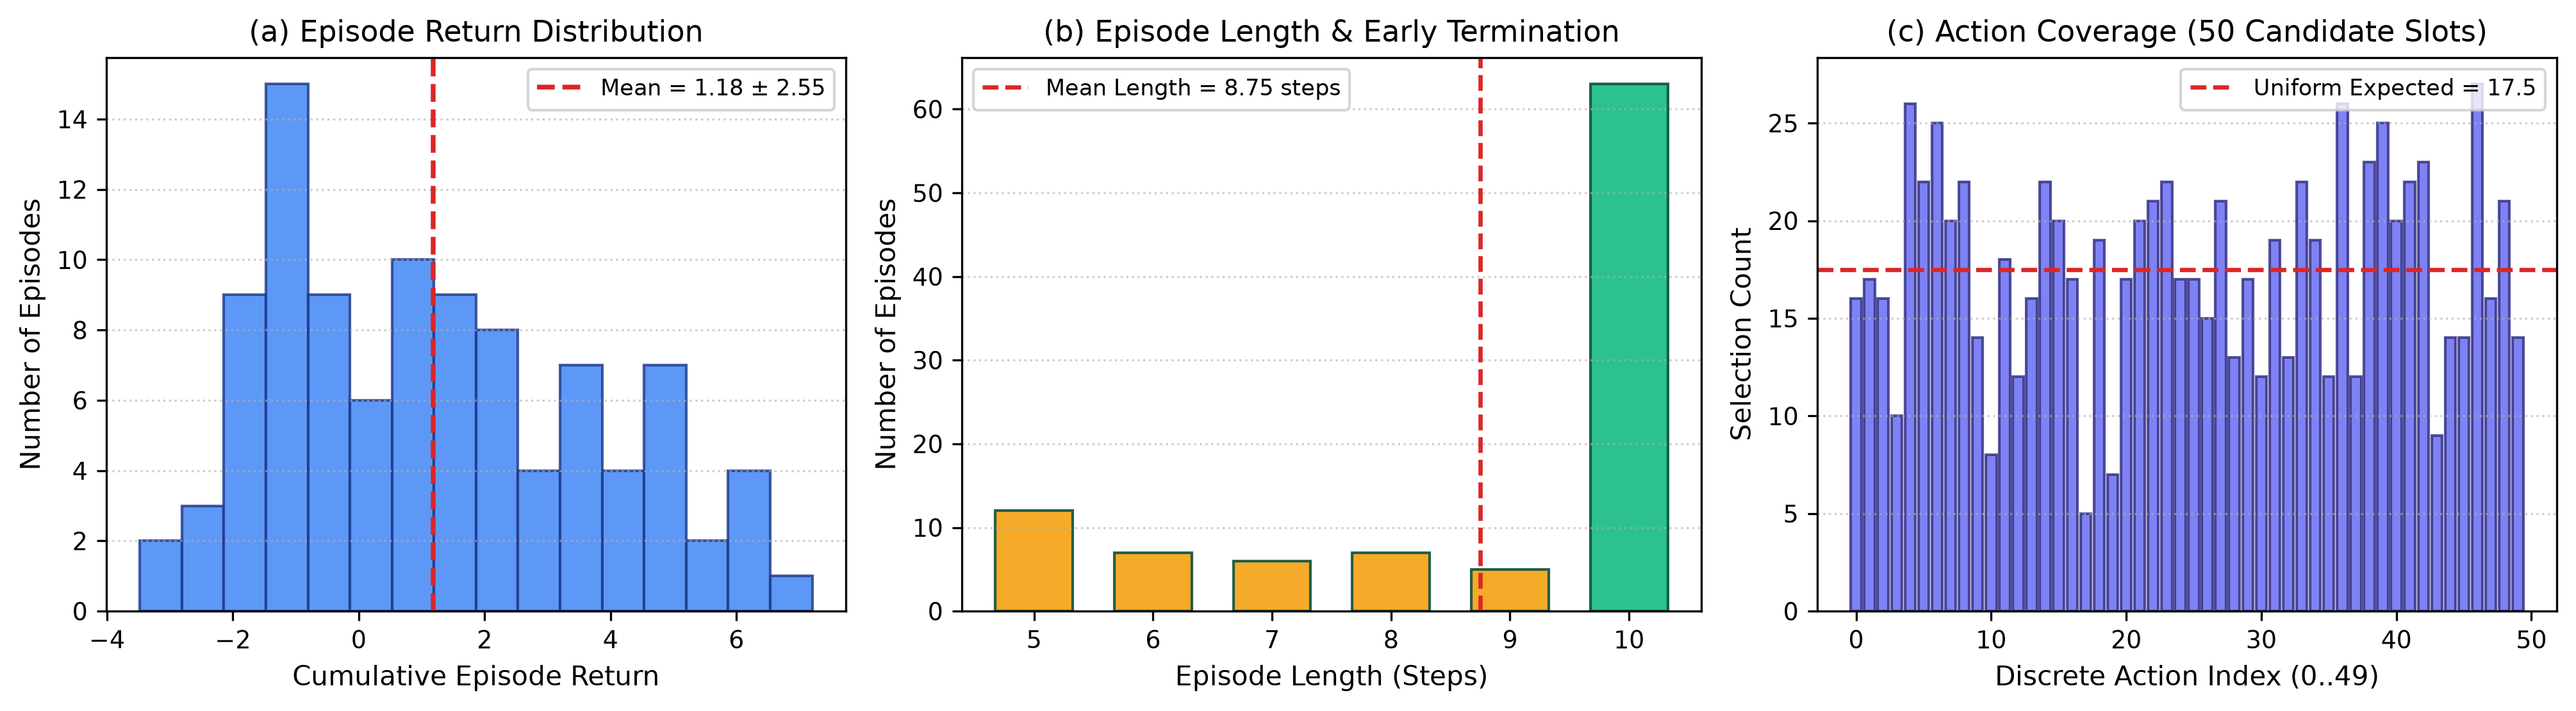
\includegraphics[width=0.96\textwidth]{figures/fig2_random_policy_diagnostics.png}
    \caption{Random-policy environment validation diagnostics across $N = 100$ episodes ($875$ total interaction steps): (a) Cumulative episode return distribution centered at $1.1833 \pm 2.5468$ over $[-3.4769, 7.2058]$, confirming a well-scaled reward landscape without trivial saturation; (b) Episode length histogram showing a $37.0\%$ early termination rate between steps $t=5$ and $t=9$ due to the $5$-consecutive-miss user abandonment rule versus $63.0\%$ full $10$-step horizon completion (mean length $8.75 \pm 1.85$ steps); and (c) Discrete action selection counts across all $50$ candidate slots relative to the theoretical uniform expectation ($17.5$ selections/slot), confirming $100\%$ action-space reachability ($50/50$ unique actions sampled).}
    \label{fig:random_diag}
\end{figure*}

Three structural properties emerge from Table~\ref{tab:random_diag} and Fig.~\ref{fig:random_diag}:
\begin{enumerate}
    \item \textbf{Well-Scaled Reward Landscape:} As shown in Fig.~\ref{fig:random_diag}(a), unguided uniform action selection yields a mean cumulative episode return of $1.1833 \pm 2.5468$, spanning a wide dynamic range from $-3.4769$ (sessions dominated by irrelevant recommendations, repetition penalties, and early abandonment) to $7.2058$ (fortuitous sequences of relevant and novel items). The step-level hit rate of $0.3053$ confirms that roughly $30.53\%$ of candidate pool slots correspond to positive user preferences, providing sufficient positive reinforcement signal for initial $\epsilon$-greedy exploration without making the task trivially solvable.
    \item \textbf{Active Session Abandonment Dynamics:} Fig.~\ref{fig:random_diag}(b) demonstrates that $37.0\%$ of random episodes terminate prematurely ($t \in \{5, 6, 7, 8, 9\}$) upon accumulating $5$ consecutive negative interactions, while $63.0\%$ survive to the full $H=10$ horizon, yielding a mean episode length of $8.75 \pm 1.85$ steps. This confirms that the user abandonment rule actively penalizes myopic or repetitive policies and incentivizes multi-step survival planning.
    \item \textbf{Complete Candidate Action Reachability:} Across the $875$ total steps, the random policy achieves a mean self-information novelty of $14.39$ bits ($14.3890$ bits), a repeat action rate of $7.89\%$ ($0.0789$), and samples all $50/50$ ($100\%$) discrete candidate slots around the theoretical uniform expectation of $875 / 50 = 17.5$ selections per slot (Fig.~\ref{fig:random_diag}(c)). This verifies that no candidate slots are structurally masked or unreachable prior to policy optimization.
\end{enumerate}

\subsection{Hyperparameter Sensitivity and Training Dynamics}
\label{subsec:hyperparam}

To systematically evaluate the stability and sample efficiency of our D3QN architecture, we conducted a controlled one-factor-at-a-time hyperparameter sensitivity study across eight configurations (\texttt{cfg1\_baseline} through \texttt{cfg8\_high\_l2}), each trained for $800$ episodes around the baseline setting ($\eta = 5 \times 10^{-4}$, $\gamma = 0.95$, $\delta_\epsilon = 0.995$, $\lambda_{L_2} = 10^{-5}$). Based on the sensitivity findings, we subsequently trained our Champion Tuned D3QN (\texttt{d3qn\_tuned}) for an extended schedule of $1{,}500$ episodes ($14{,}940$ total environment interaction steps). Table~\ref{tab:hyperparams} reports the complete validation metrics across all nine runs, while Fig.~\ref{fig:hyperparams} and Fig.~\ref{fig:exploration} illustrate the validation learning curves, hyperparameter sensitivity comparison, and internal value-function convergence dynamics.

\begin{table*}[t]
\centering
\caption{Hyperparameter Sensitivity Study ($800$ Episodes) and Champion Tuned D3QN ($1{,}500$ Episodes, $14{,}940$ Steps) on Validation Split ($H = 10$)}
\label{tab:hyperparams}
\resizebox{\textwidth}{!}{%
\begin{tabular}{@{}lccccccccccc@{}}
\toprule
\textbf{Configuration ID} & \textbf{LR $\eta$} & \textbf{Discount $\gamma$} & \textbf{Decay $\delta_\epsilon$} & \textbf{$L_2$ $\lambda_{L_2}$} & \textbf{Episodes} & \textbf{Final Val Return} & \textbf{Best Val Return} & \textbf{Val P@10} & \textbf{NDCG@10} & \textbf{MAP@10} & \textbf{Catalog Coverage} \\
\midrule
\texttt{cfg1\_baseline} & $5\times 10^{-4}$ & $0.95$ & $0.995$ & $10^{-5}$ & $800$ & $11.6598$ & $11.6598$ & $0.9490$ & $0.9610$ & $0.9348$ & $\mathbf{0.3586}$ ($\mathbf{35.86\%}$) \\
\texttt{cfg2\_high\_lr} & $1\times 10^{-3}$ & $0.95$ & $0.995$ & $10^{-5}$ & $800$ & $10.0227$ & $10.2034$ & $0.8410$ & $0.8609$ & $0.7799$ & $0.3433$ ($34.33\%$) \\
\texttt{cfg3\_low\_lr} & $1\times 10^{-4}$ & $0.95$ & $0.995$ & $10^{-5}$ & $800$ & $9.7503$ & $9.7503$ & $0.8220$ & $0.8630$ & $0.7758$ & $0.3533$ ($35.33\%$) \\
\texttt{cfg4\_gamma\_090} & $5\times 10^{-4}$ & $0.90$ & $0.995$ & $10^{-5}$ & $800$ & $11.3549$ & $11.4411$ & $0.9280$ & $0.9470$ & $0.9093$ & $0.3528$ ($35.28\%$) \\
\texttt{cfg5\_gamma\_099} & $5\times 10^{-4}$ & $0.99$ & $0.995$ & $10^{-5}$ & $800$ & $11.0368$ & $11.0368$ & $0.9030$ & $0.9196$ & $0.8655$ & $0.3454$ ($34.54\%$) \\
\texttt{cfg6\_fast\_eps} & $5\times 10^{-4}$ & $0.95$ & $0.990$ & $10^{-5}$ & $800$ & $11.5811$ & $11.5811$ & $0.9420$ & $0.9515$ & $0.9179$ & $0.3444$ ($34.44\%$) \\
\texttt{cfg7\_slow\_eps} & $5\times 10^{-4}$ & $0.95$ & $0.998$ & $10^{-5}$ & $800$ & $11.5718$ & $11.6073$ & $0.9360$ & $0.9438$ & $0.9085$ & $0.3470$ ($34.70\%$) \\
\texttt{cfg8\_high\_l2} & $5\times 10^{-4}$ & $0.95$ & $0.995$ & $10^{-4}$ & $800$ & $11.4517$ & $11.4517$ & $0.9350$ & $0.9514$ & $0.9153$ & $0.3486$ ($34.86\%$) \\
\midrule
\texttt{d3qn\_tuned} (Champion) & $5\times 10^{-4}$ & $0.95$ & $0.995$ & $10^{-5}$ & $1{,}500$ & $\mathbf{12.1668}$ & $\mathbf{12.2125}$ & $\mathbf{0.9770}$ & $\mathbf{0.9807}$ & $\mathbf{0.9684}$ & $0.3465$ ($34.65\%$) \\
\bottomrule
\end{tabular}%
}
\end{table*}

\begin{figure*}[t]
    \centering
    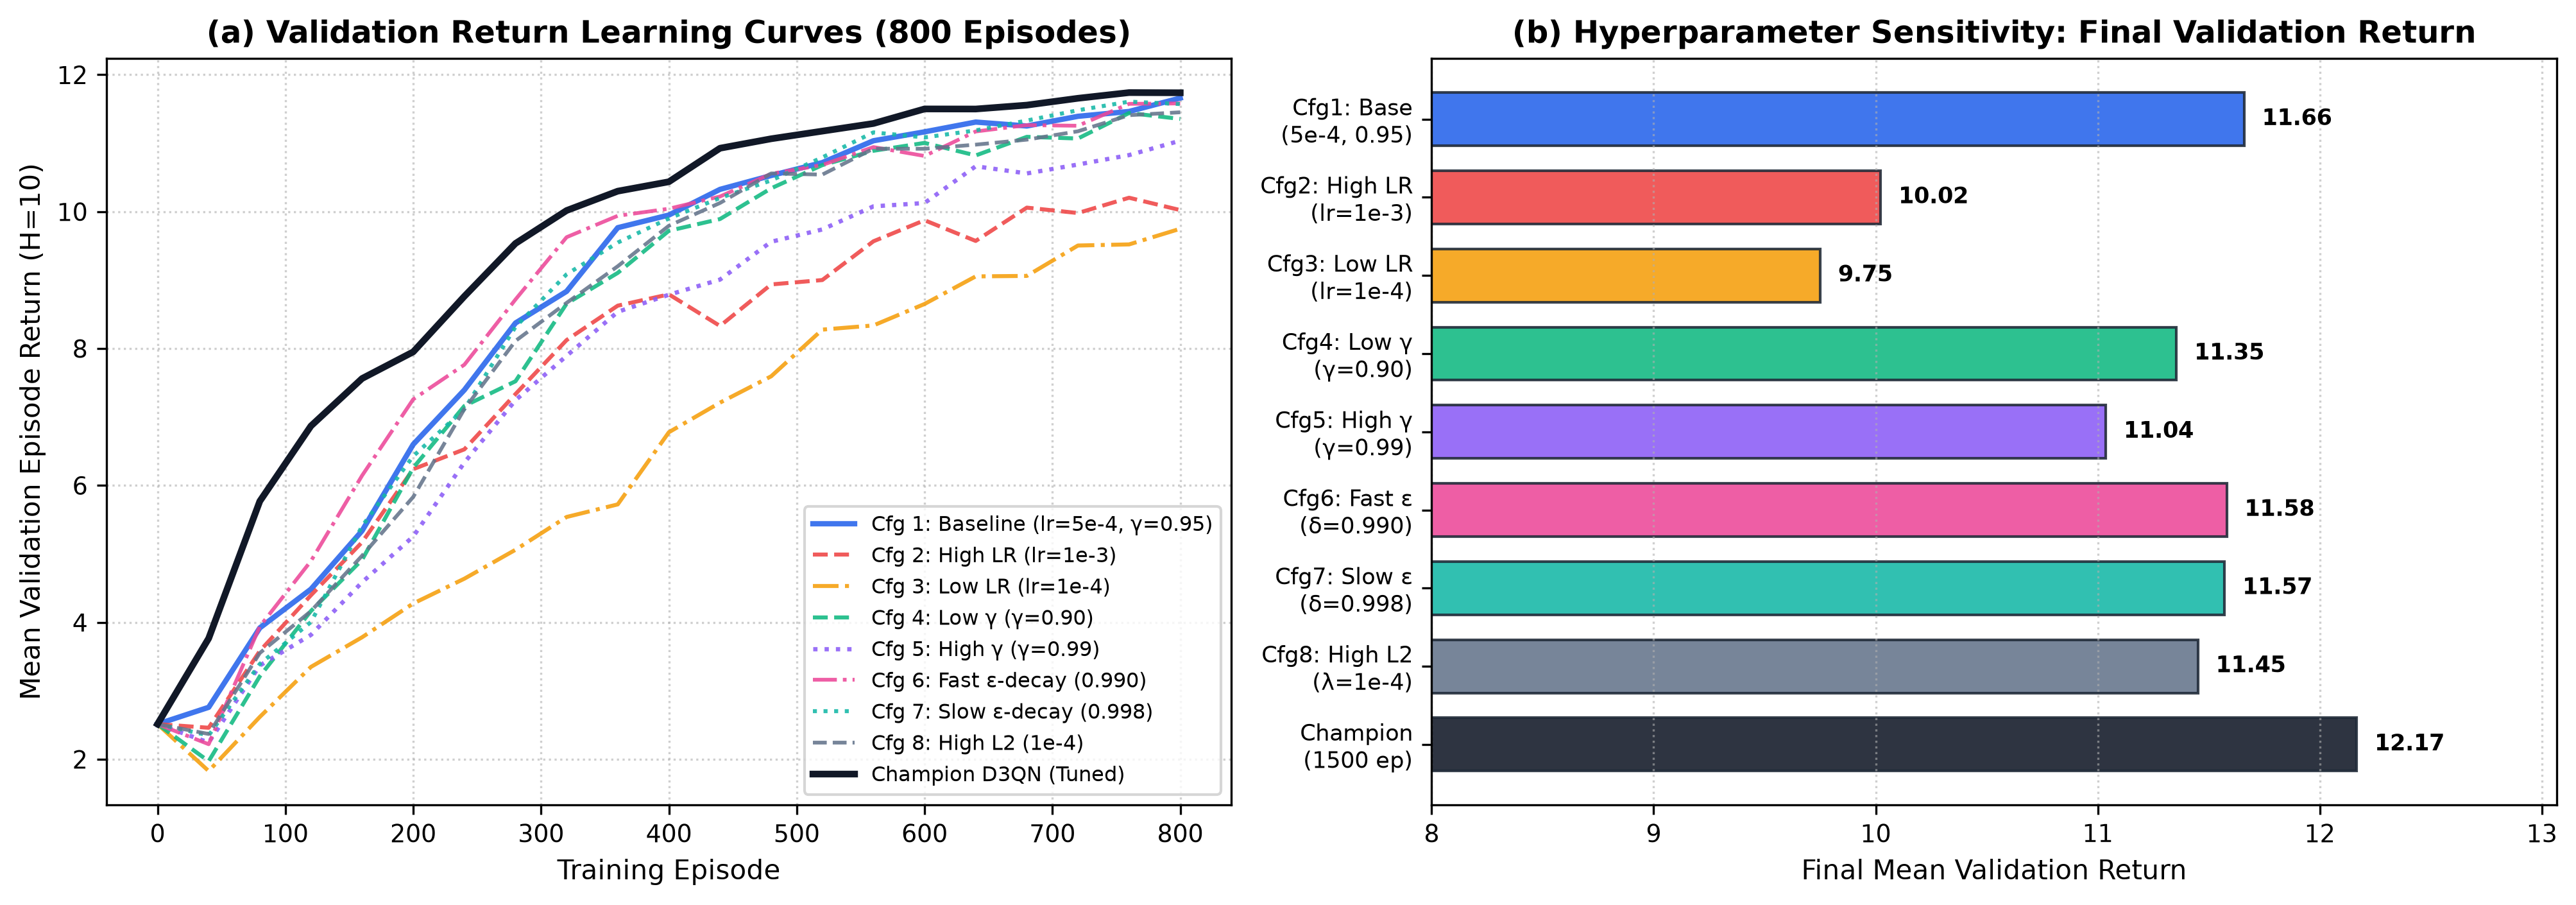
\includegraphics[width=0.96\textwidth]{figures/fig3_hyperparameter_learning_curves.png}
    \caption{Hyperparameter sensitivity analysis across $800$ training episodes and extended Champion D3QN training ($1{,}500$ episodes): (a) Mean validation episode return learning curves ($H=10$, evaluated every $40$ episodes at $\epsilon=0$), showing rapid convergence for $\eta = 5 \times 10^{-4}$ and $\gamma = 0.95$ compared to high-LR oscillation ($\eta = 10^{-3}$) and low-LR under-fitting ($\eta = 10^{-4}$); and (b) Final validation return comparison across all eight $800$-episode configurations and the Champion Tuned D3QN ($12.1668$).}
    \label{fig:hyperparams}
\end{figure*}

\begin{figure*}[t]
    \centering
    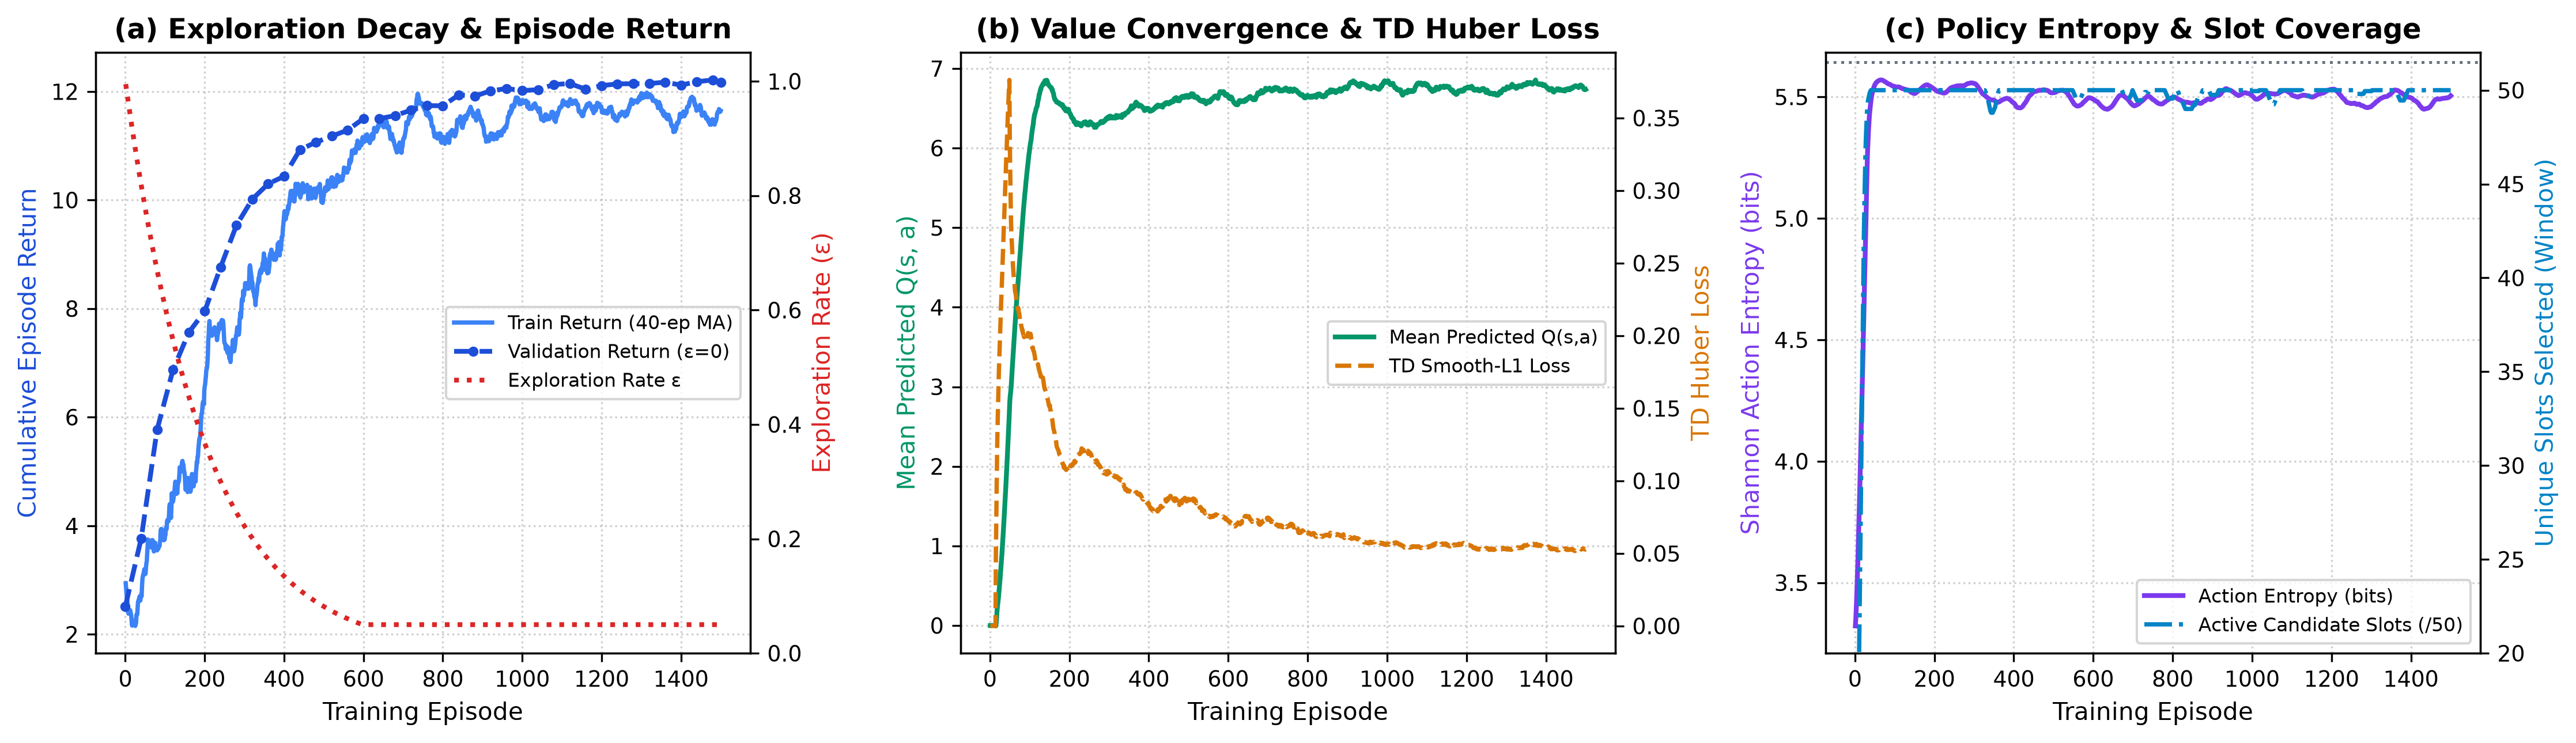
\includegraphics[width=0.96\textwidth]{figures/fig4_exploration_dynamics.png}
    \caption{Internal training and exploration dynamics of the Champion Tuned D3QN across $1{,}500$ episodes ($14{,}940$ steps): (a) Co-evolution of the $40$-episode moving-average training return, greedy validation return ($\epsilon=0$), and exponential exploration rate $\epsilon_t$; (b) Stabilization of mean predicted action-values $Q(s,a)$ alongside the monotonic decay of temporal-difference (TD) Smooth-$L_1$ (Huber) loss; and (c) Policy Shannon action entropy (bits) and sliding-window active candidate slot coverage ($50/50$ slots).}
    \label{fig:exploration}
\end{figure*}

\paragraph{Learning Rate Sensitivity ($\eta$)}
As evidenced in Table~\ref{tab:hyperparams} and Fig.~\ref{fig:hyperparams}(a), the AdamW step size $\eta$ exerts the strongest influence on policy convergence. The moderate learning rate $\eta = 5 \times 10^{-4}$ (\texttt{cfg1\_baseline}) achieves the highest $800$-episode performance across all ranking and return criteria, reaching a final validation return of $11.6598$, P@10 of $0.9490$, NDCG@10 of $0.9610$, MAP@10 of $0.9348$, and the highest validation catalog coverage of $0.3586$ ($35.86\%$). Increasing the step size to $\eta = 10^{-3}$ (\texttt{cfg2\_high\_lr}) degrades final validation return to $10.0227$ (best $10.2034$, NDCG@10 of $0.8609$, MAP@10 of $0.7799$) because aggressive gradient updates amplify moving-target non-stationarity in the Polyak-averaged target network, inducing target $Q$-value overshoot and mid-training return oscillations after episode $350$. Conversely, reducing the learning rate to $\eta = 10^{-4}$ (\texttt{cfg3\_low\_lr}) yields the lowest validation return of $9.7503$ (P@10 of $0.8220$, NDCG@10 of $0.8630$, MAP@10 of $0.7758$), as parameter updates proceed too slowly to separate the advantage stream $A_\theta(s,a)$ across the $50$ candidate slots within an $800$-episode budget.

\paragraph{Discount Factor Sensitivity ($\gamma$)}
Varying the Bellman discount factor confirms the necessity of multi-step trajectory planning over myopic or over-extended horizons. Setting $\gamma = 0.95$ (\texttt{cfg1\_baseline}, validation return $11.6598$) outperforms both a more myopic discount of $\gamma = 0.90$ (\texttt{cfg4\_gamma\_090}, final validation return $11.3549$, best $11.4411$, P@10 of $0.9280$, NDCG@10 of $0.9470$) and a near-undiscounted $\gamma = 0.99$ (\texttt{cfg5\_gamma\_099}, final validation return $11.0368$, P@10 of $0.9030$, NDCG@10 of $0.9196$). Under $\gamma = 0.90$, the effective planning horizon $(1-\gamma)^{-1} = 10$ steps heavily discounts late-session diversity and novelty rewards, leading to premature genre saturation. Conversely, $\gamma = 0.99$ propagates long-horizon bootstrap variance across episodes of length $H=10$, destabilizing Bellman target estimation and depressing MAP@10 to $0.8655$.

\paragraph{Exploration Schedule ($\delta_\epsilon$) and $L_2$ Regularization ($\lambda_{L_2}$)}
Faster exploration decay $\delta_\epsilon = 0.990$ (\texttt{cfg6\_fast\_eps}) accelerates early validation gains between episodes $100$ and $350$ (Fig.~\ref{fig:hyperparams}(a)) and finishes at $11.5811$ (NDCG@10 of $0.9515$), but its premature transition to greedy exploitation slightly narrows catalog coverage to $0.3444$ ($34.44\%$). Slower decay $\delta_\epsilon = 0.998$ (\texttt{cfg7\_slow\_eps}) maintains prolonged stochasticity, achieving a best validation return of $11.6073$ (final $11.5718$, NDCG@10 of $0.9438$) and higher validation novelty ($15.4025$ bits), at the cost of slower initial convergence. Stronger weight decay $\lambda_{L_2} = 10^{-4}$ (\texttt{cfg8\_high\_l2}) regularizes network weights slightly too aggressively, yielding a final validation return of $11.4517$ (P@10 of $0.9350$, NDCG@10 of $0.9514$) compared to $\lambda_{L_2} = 10^{-5}$ ($11.6598$).

\paragraph{Champion Tuned D3QN Convergence and Sample Efficiency}
Retaining the optimal hyperparameters ($\eta = 5 \times 10^{-4}$, $\gamma = 0.95$, $\delta_\epsilon = 0.995$, $\lambda_{L_2} = 10^{-5}$) over $1{,}500$ episodes ($14{,}940$ steps) allows the Champion Tuned D3QN (\texttt{d3qn\_tuned}) to reach a final validation return of $12.1668$ (peaking at a best validation return of $12.2125$ at episode $1{,}480$ / step $14{,}740$), alongside a validation P@10 of $0.9770$, R@10 of $0.5147$, NDCG@10 of $0.9807$, MAP@10 of $0.9684$, HR@10 of $1.0000$, catalog coverage of $0.3465$ ($34.65\%$), and mean novelty of $15.5923$ bits. As shown in Fig.~\ref{fig:exploration}(a), the agent exhibits exceptional sample efficiency: starting from an untrained return of $2.5138$ at step $0$ (which already exceeds the static Greedy FunkSVD baseline of $1.3609$ due to hybrid candidate generation), the D3QN policy surpasses the Myopic Contextual Bandit return threshold ($10.4924$) after just $3{,}940$ interaction steps ($400$ episodes, validation return $10.4368 \to 10.9268$ at episode $440$). Fig.~\ref{fig:exploration}(b) confirms that Double DQN decoupling and dueling value-advantage decomposition prevent maximization bias: the mean predicted $Q(s,a)$ converges smoothly to an asymptotic plateau near $6.75$ while the TD Smooth-$L_1$ (Huber) loss decays monotonically from an initial peak of $0.38$ to a stable floor of $0.05$. Simultaneously, Fig.~\ref{fig:exploration}(c) shows that policy Shannon entropy stabilizes near $5.50$ bits (close to the $\log_2 50 \approx 5.6439$-bit uniform ceiling across users) while utilizing all $50/50$ candidate slots.

\subsection{Test-Set Evaluation and Baseline Comparison}
\label{subsec:test_eval}

We evaluated the locked Champion D3QN policy ($\epsilon = 0$) against five baselines across all $250$ held-out test users under two recommendation horizons: $K = 10$ ($H = 10$ steps) and $K = 20$ ($H = 20$ steps). The evaluated baselines span unguided selection (\texttt{Random}), non-personalized and additive-bias heuristics (\texttt{Popularity} and \texttt{Bias} $\mu + b_u + b_i$), our Workshop~1 matrix factorization model deployed sequentially (\texttt{Greedy FunkSVD}), and a neural contextual bandit trained with identical state-action representations but zero lookahead (\texttt{Myopic Contextual Bandit}, $\gamma = 0$). Table~\ref{tab:test_comparison} details the complete test-set performance across nine evaluation metrics, and Fig.~\ref{fig:test_comparison} visualizes the top-$10$ ranking accuracy and the multi-objective accuracy--coverage--novelty trade-off.

\begin{table*}[t]
\centering
\caption{Comprehensive Test-Set Evaluation Across $250$ Held-Out Users at Horizons $K = 10$ and $K = 20$}
\label{tab:test_comparison}
\resizebox{\textwidth}{!}{%
\begin{tabular}{@{}clccccccccc@{}}
\toprule
\textbf{Horizon} & \textbf{Policy / Model} & \textbf{Mean Return ($\pm$ SD)} & \textbf{P@$K$} & \textbf{R@$K$} & \textbf{NDCG@$K$} & \textbf{MAP@$K$} & \textbf{HR@$K$} & \textbf{Catalog Cov. (\%)} & \textbf{Novelty (bits)} & \textbf{ILD} \\
\midrule
$K = 10$ & Random & $2.6805 \pm 2.4628$ & $0.3412$ & $0.1798$ & $0.3480$ & $0.1949$ & $0.9080$ & $\mathbf{43.48\%}$ & $14.7450$ & $\mathbf{0.9664}$ \\
$K = 10$ & Bias ($\mu + b_u + b_i$) & $-0.0451 \pm 1.7509$ & $0.1188$ & $0.0626$ & $0.1345$ & $0.0658$ & $0.5000$ & $7.93\%$ & $14.5493$ & $0.8030$ \\
$K = 10$ & Popularity & $-1.4121 \pm 0.6586$ & $0.0392$ & $0.0207$ & $0.0551$ & $0.0240$ & $0.2800$ & $4.02\%$ & $8.8545$ & $0.6864$ \\
$K = 10$ & Greedy FunkSVD (Workshop 1) & $1.3609 \pm 2.1743$ & $0.2524$ & $0.1330$ & $0.2785$ & $0.1519$ & $0.7920$ & $17.25\%$ & $13.0788$ & $0.8653$ \\
$K = 10$ & Myopic Contextual Bandit ($\gamma=0$) & $10.4924 \pm 1.8230$ & $0.8708$ & $0.4589$ & $0.8924$ & $0.8253$ & $\mathbf{1.0000}$ & $34.35\%$ & $14.9406$ & $0.4215$ \\
$K = 10$ & \textbf{D3QN (Ours, $\gamma=0.95$)} & $\mathbf{12.3674 \pm 0.8253}$ & $\mathbf{0.9792}$ & $\mathbf{0.5160}$ & $\mathbf{0.9818}$ & $\mathbf{0.9692}$ & $\mathbf{1.0000}$ & $36.64\%$ & $\mathbf{17.9613}$ & $0.2731$ \\
\midrule
$K = 20$ & Random & $4.3195 \pm 3.2988$ & $0.2954$ & $0.3113$ & $0.3274$ & $0.1610$ & $0.9280$ & $59.19\%$ & $14.5759$ & $\mathbf{0.9734}$ \\
$K = 20$ & Bias ($\mu + b_u + b_i$) & $-0.0470 \pm 1.9373$ & $0.0766$ & $0.0807$ & $0.1028$ & $0.0415$ & $0.5000$ & $12.36\%$ & $14.3013$ & $0.8009$ \\
$K = 20$ & Popularity & $-1.4224 \pm 0.7428$ & $0.0210$ & $0.0222$ & $0.0379$ & $0.0132$ & $0.2800$ & $4.51\%$ & $8.8756$ & $0.6862$ \\
$K = 20$ & Greedy FunkSVD (Workshop 1) & $1.4372 \pm 2.6229$ & $0.1616$ & $0.1704$ & $0.2127$ & $0.0959$ & $0.7920$ & $25.10\%$ & $13.2404$ & $0.8742$ \\
$K = 20$ & Myopic Contextual Bandit ($\gamma=0$) & $16.5601 \pm 4.1903$ & $0.7262$ & $0.7654$ & $0.8068$ & $0.6852$ & $\mathbf{1.0000}$ & $57.42\%$ & $15.9685$ & $0.6061$ \\
$K = 20$ & \textbf{D3QN (Ours, $\gamma=0.95$)} & $\mathbf{20.1006 \pm 1.8207}$ & $\mathbf{0.8398}$ & $\mathbf{0.8849}$ & $\mathbf{0.9167}$ & $\mathbf{0.8605}$ & $\mathbf{1.0000}$ & $\mathbf{60.35\%}$ & $\mathbf{17.2745}$ & $0.4698$ \\
\bottomrule
\end{tabular}%
}
\end{table*}

\begin{figure*}[t]
    \centering
    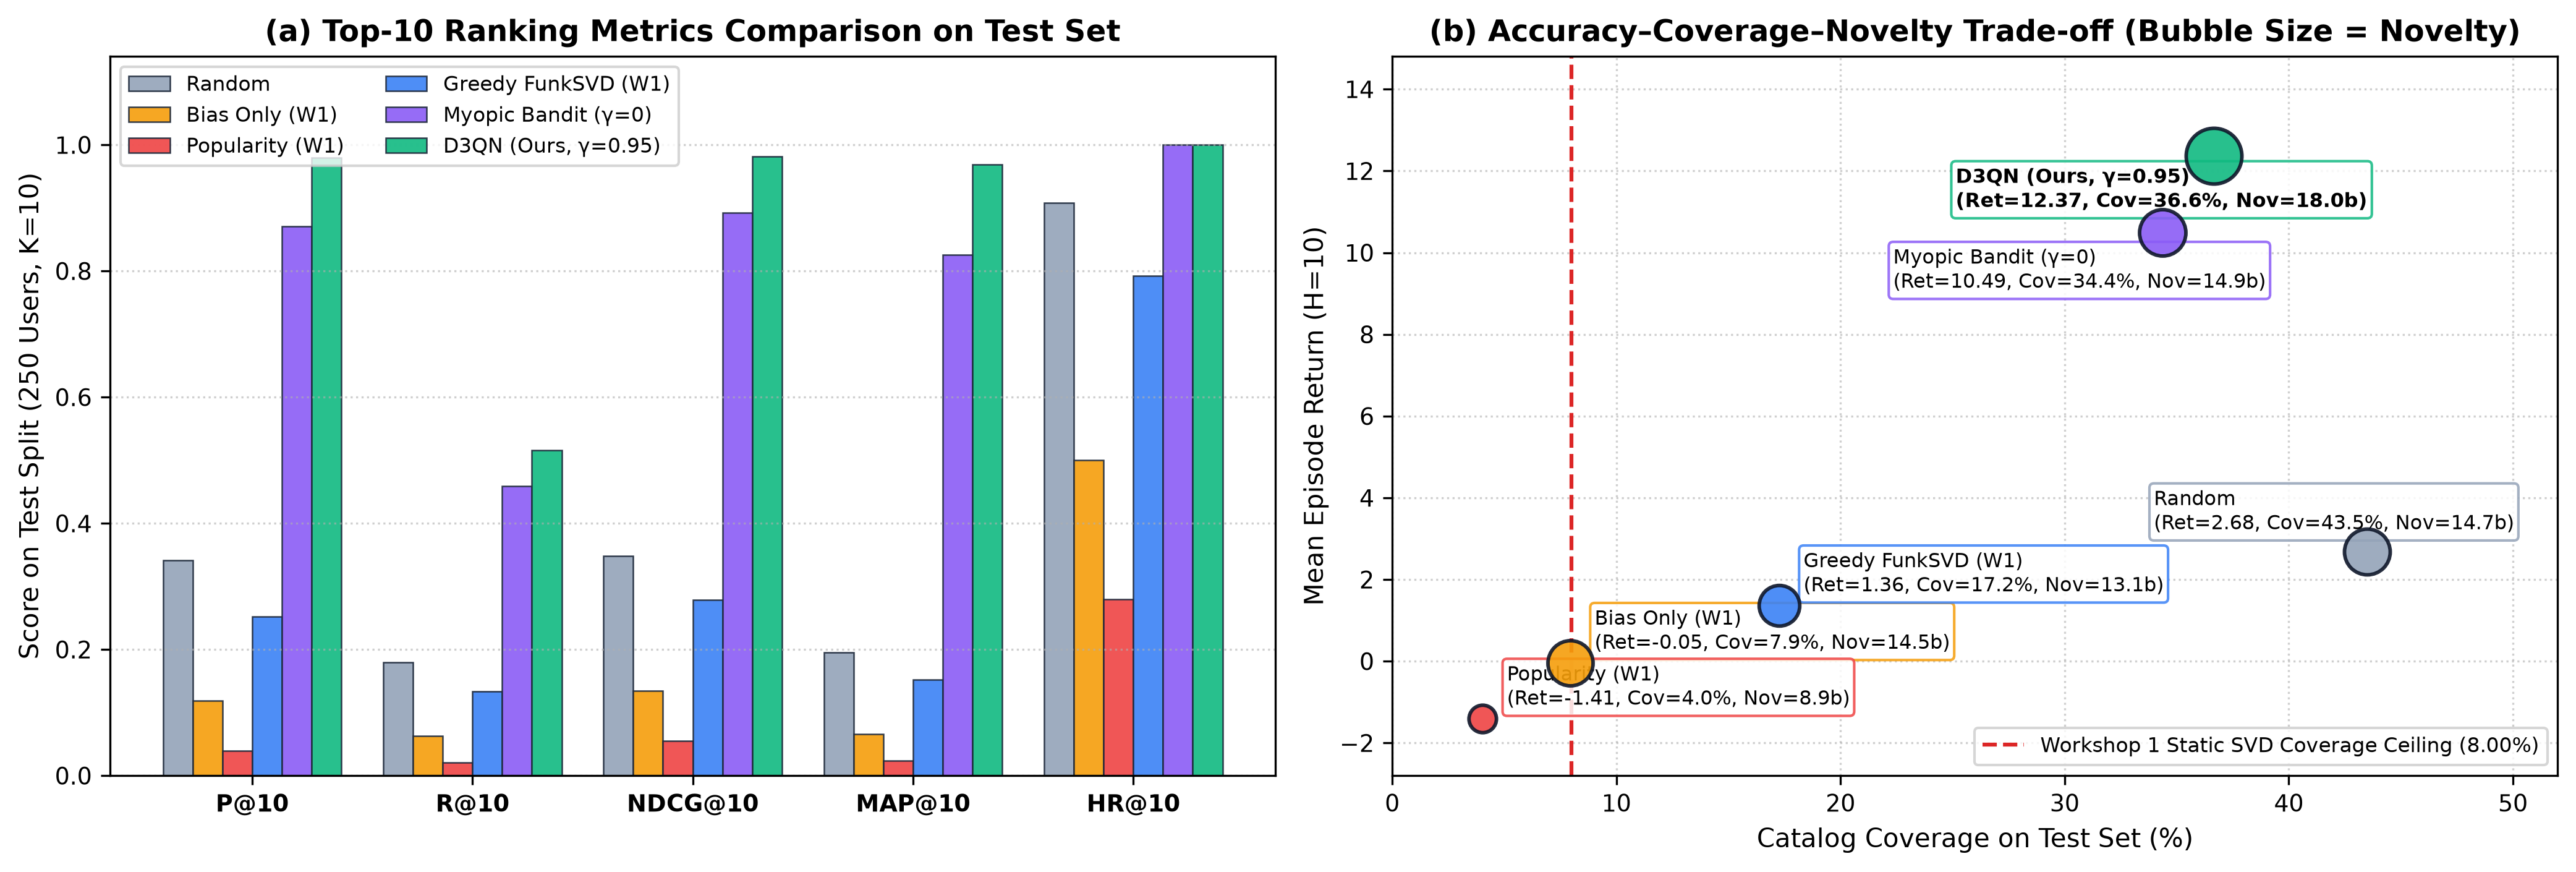
\includegraphics[width=0.96\textwidth]{figures/fig5_test_metrics_comparison.png}
    \caption{Test-set evaluation across $250$ held-out users: (a) Top-$10$ ranking metrics comparison (P@10, R@10, NDCG@10, MAP@10, and HR@10), illustrating the progression from static Workshop~1 baselines (\texttt{Popularity}, \texttt{Bias Only}, \texttt{Greedy FunkSVD}) to the \texttt{Myopic Bandit} ($\gamma=0$) and our proposed \texttt{D3QN} ($\gamma=0.95$); and (b) Multi-objective accuracy--coverage--novelty trade-off at $K=10$ (bubble area proportional to self-information novelty in bits), showing how D3QN simultaneously maximizes mean return ($12.3674$) and novelty ($17.96$ bits) while expanding catalog coverage to $36.64\%$ ($4.58\times$ the $8.00\%$ Workshop~1 static SVD ceiling).}
    \label{fig:test_comparison}
\end{figure*}

\paragraph{Superior Sequential Ranking and Trajectory Return}
Across both evaluation horizons in Table~\ref{tab:test_comparison}, \texttt{D3QN (Ours)} substantially outperforms every baseline on cumulative return, ranking precision, discounted ranking quality, and item novelty. At $K = 10$, D3QN achieves a mean episode return of $12.3674 \pm 0.8253$ (with $100\%$ of sessions completing the full $10.0$-step horizon), P@10 of $0.9792$, R@10 of $0.5160$, NDCG@10 of $0.9818$, MAP@10 of $0.9692$, and HR@10 of $1.0000$. When the evaluation horizon doubles to $K = 20$ without retraining, D3QN maintains full $20.0$-step session survival across all $250$ users, reaching a mean return of $20.1006 \pm 1.8207$, P@20 of $0.8398$, R@20 of $0.8849$, NDCG@20 of $0.9167$, MAP@20 of $0.8605$, and HR@20 of $1.0000$ (while its top-$10$ prefix metrics inside the $H=20$ rollout reach P@10 $= 0.9796$, R@10 $= 0.5162$, NDCG@10 $= 0.9825$, and MAP@10 $= 0.9707$).

\paragraph{Failure of Static Heuristics and Greedy Matrix Factorization in Sequential Interaction}
A striking empirical finding in Table~\ref{tab:test_comparison} and Fig.~\ref{fig:test_comparison}(a) is the severe degradation of static recommenders when deployed in an interactive sequential environment. In our Workshop~1 static offline evaluation, matrix factorization (\texttt{FunkSVD}) achieved a competitive rating prediction accuracy of $\text{RMSE} = 0.8041$ ($0.8128$ on the global unpooled split), yet suffered from the classic accuracy--ranking mismatch: on global all-item ranking, \texttt{Popularity} achieved NDCG@10 of $0.6726$ versus \texttt{FunkSVD}'s $0.5881$ ($0.2460$ on the Workshop~1 static test split with P@10 $= 0.2190$, R@10 $= 0.1450$, MAP@10 $= 0.1440$, HR@10 $= 0.5620$, novelty $= 9.83$ bits, and catalog coverage capped at only $8.00\%$). In the sequential MDP environment of Workshop~3, repeatedly selecting head items (\texttt{Popularity}) or static baseline scores (\texttt{Bias} $\mu + b_u + b_i$) fails to adapt to user feedback and rapidly triggers the $5$-consecutive-miss abandonment rule: at $K=10$, \texttt{Popularity} averages only $5.8720$ steps per episode with a negative mean return of $-1.4121 \pm 0.6586$ (P@10 $= 0.0392$, NDCG@10 $= 0.0551$, coverage $= 4.02\%$, novelty $= 8.8545$ bits), while \texttt{Bias} terminates at $6.9360$ steps with a mean return of $-0.0451 \pm 1.7509$ (P@10 $= 0.1188$, NDCG@10 $= 0.1345$, coverage $= 7.93\%$). Even \texttt{Greedy FunkSVD}, which ranks candidates strictly by static dot-product predictions $\hat{r}_{u,i}$ without state evolution, achieves a mean return of only $1.3609 \pm 2.1743$ at $K=10$ (mean length $8.5000$ steps, P@10 $= 0.2524$, R@10 $= 0.1330$, NDCG@10 $= 0.2785$, MAP@10 $= 0.1519$, coverage $= 17.25\%$) and $1.4372 \pm 2.6229$ at $K=20$ (mean length $11.7200$ steps, P@20 $= 0.1616$, NDCG@20 $= 0.2127$). Because \texttt{Greedy FunkSVD} lacks negative preference suppression and novelty planning, it underperforms even the memoryless \texttt{Random} policy ($2.6805$ at $K=10$ and $4.3195$ at $K=20$), which naturally avoids deterministic failure loops through uniform slot sampling.

\paragraph{Value of Multi-Step Bellman Planning ($\gamma = 0.95$ vs.\ Myopic Bandit $\gamma = 0$)}
Comparing \texttt{D3QN} ($\gamma = 0.95$) against the \texttt{Myopic Contextual Bandit} ($\gamma = 0$) isolates the exact contribution of multi-step Bellman lookahead, since both models observe the identical $250$-dimensional state representation across the $50$ candidate slots. At $K=10$, multi-step planning increases mean episode return by $+17.87\%$ ($12.3674$ vs.\ $10.4924$) while cutting return standard deviation more than in half ($0.8253$ vs.\ $1.8230$), boosting P@10 from $0.8708$ to $0.9792$ ($+10.84$ percentage points), NDCG@10 from $0.8924$ to $0.9818$ ($+8.94$ points), and MAP@10 from $0.8253$ to $0.9692$ ($+14.39$ points). The advantage of long-horizon planning becomes even more pronounced at $K = 20$: while the myopic bandit begins to exhaust obvious high-scoring candidates and suffers early terminations (mean length dropping to $19.5200$ steps, return $16.5601 \pm 4.1903$, P@20 $= 0.7262$, NDCG@20 $= 0.8068$, MAP@20 $= 0.6852$), D3QN sustains $20.0$-step completion across every user and achieves a $+21.38\%$ higher return ($20.1006 \pm 1.8207$), $+11.36$ points higher P@20 ($0.8398$), $+10.99$ points higher NDCG@20 ($0.9167$), and $+17.53$ points higher MAP@20 ($0.8605$).

\paragraph{Breaking the Workshop 1 Catalog Coverage and Novelty Ceiling}
Finally, Fig.~\ref{fig:test_comparison}(b) highlights how sequential reinforcement learning resolves the catalog concentration bottleneck identified in Workshop~1. Whereas static FunkSVD recommendations were confined to just $8.00\%$ of the catalog with a mean novelty of $9.83$ bits, D3QN expands test-set catalog coverage to $36.64\%$ at $K=10$---a $4.58\times$ expansion over Workshop~1's $8.00\%$ ceiling---while elevating mean self-information novelty to $17.96$ bits ($17.9613$ bits vs.\ $14.9406$ bits for the Myopic Bandit and $13.0788$ bits for Greedy FunkSVD). At $K=20$, D3QN expands catalog coverage further to $60.35\%$ ($0.6035$) with $17.2745$ bits of novelty, surpassing even the uniform \texttt{Random} policy ($59.19\%$) because \texttt{Random} loses $4.0$ steps per episode on average to early abandonment ($16.0$ vs.\ $20.0$ steps). Although D3QN exhibits a lower intra-list diversity ($\text{ILD} = 0.2731$ at $K=10$ and $0.4698$ at $K=20$) than unguided \texttt{Random} ($\text{ILD} = 0.9664$ and $0.9734$), this reflects purposeful preference alignment: rather than scattering recommendations across disliked genres, D3QN concentrates within each user's positively reinforced latent taste cluster while leveraging the novelty bonus to surface high-information long-tail films across the broader catalog.

\section{Trajectory Analysis, Sample Efficiency, and Discussion}
\label{sec:discussion}

To complement the aggregate evaluation metrics presented in Section~\ref{sec:results}, this section examines the microscopic behavior of the champion Dueling Double Deep Q-Network (D3QN) agent across individual user sessions, quantifies its sample efficiency relative to supervised matrix factorization and contextual bandit baselines, and critically evaluates the architectural trade-offs and methodological limitations of our sequential recommendation framework.

\subsection{Sample Episode Trajectories and Sequential Adaptation}
\label{subsec:trajectories}

\begin{figure*}[t]
    \centering
    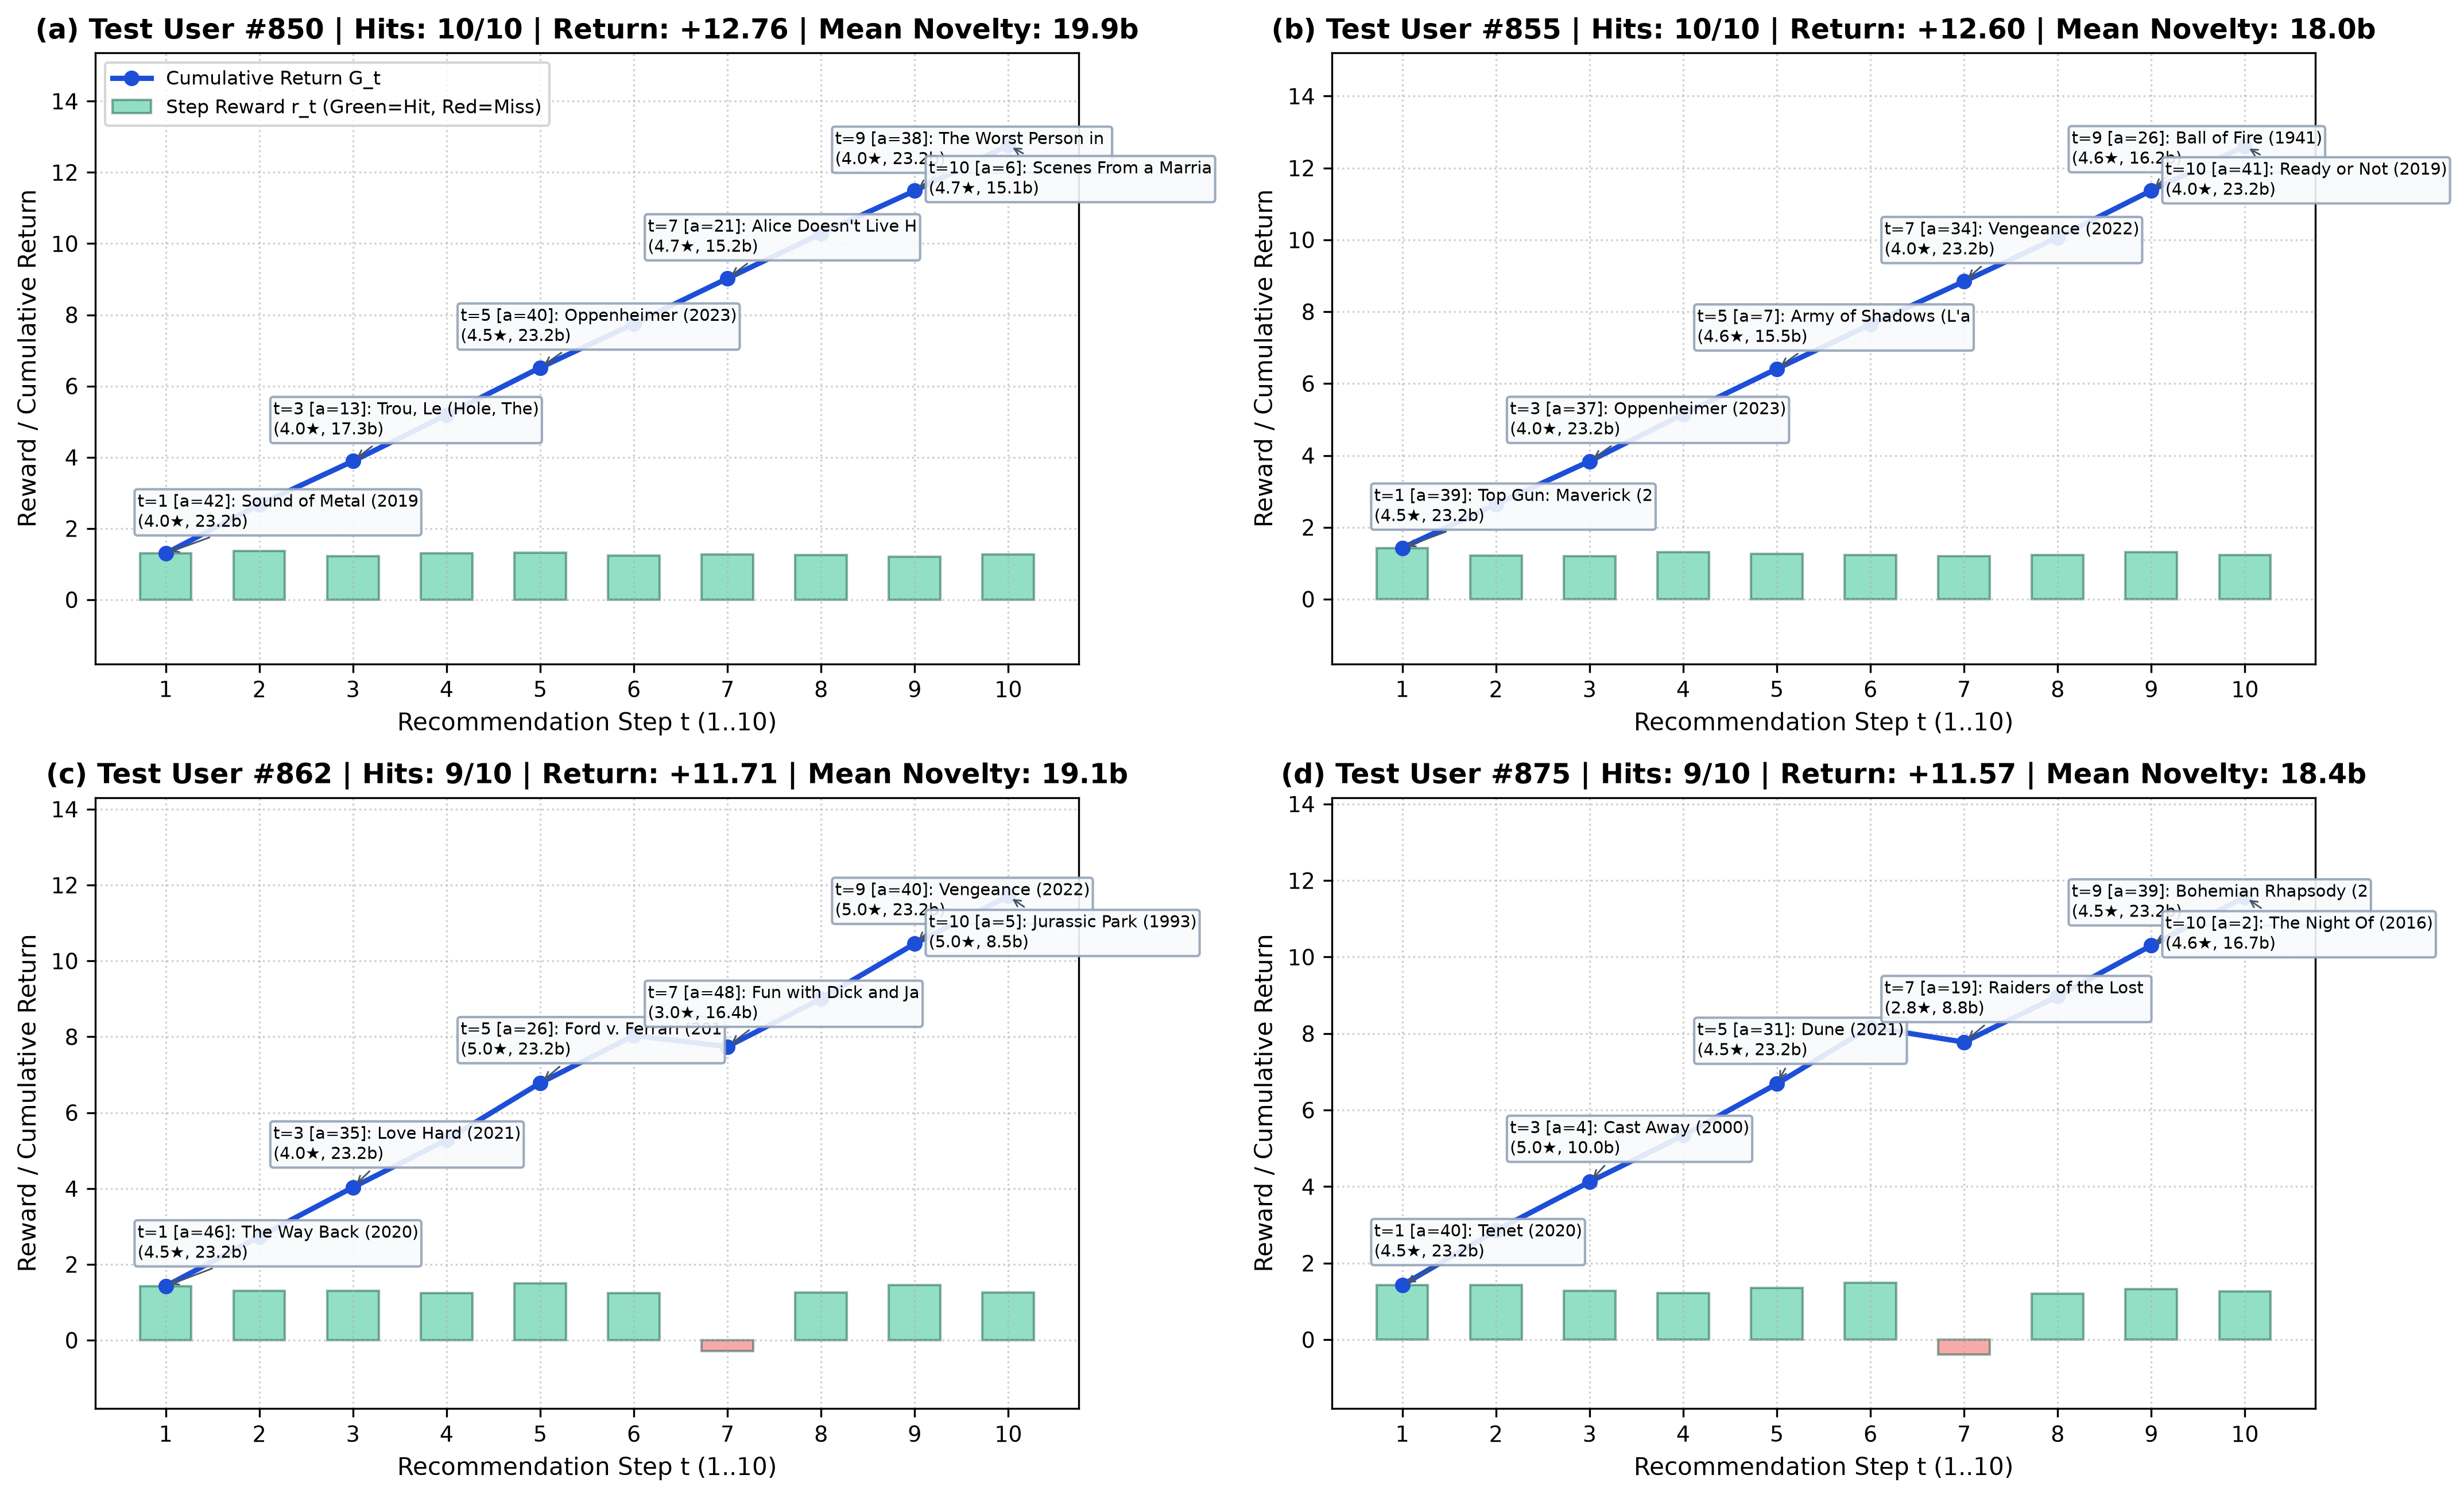
\includegraphics[width=0.96\textwidth]{figures/fig6_sample_trajectories.png}
    \caption{Step-by-step episode trajectories ($H=10$) on the held-out test split for four representative users under the champion D3QN policy. Blue curves track the cumulative undiscounted session return $G_t = \sum_{\tau=1}^{t} r_\tau$, while vertical bars indicate the immediate step reward $r_t$ (green for positive hits with $R_{u,i}^{\text{true}} \ge 3.5$, red for misses with $R_{u,i}^{\text{true}} < 3.5$). Callout annotations report the selected candidate slot $a_t \in \{0, \dots, 49\}$, movie title, ground-truth preference rating, and item self-information novelty in bits.}
    \label{fig:trajectories}
\end{figure*}

\begin{table*}[t]
    \centering
    \caption{Detailed Step-by-Step Trajectory Breakdown ($t = 1 \dots 10$) for Two Representative Held-Out Test Users under the Champion D3QN Policy: Perfect Session Execution (User \#850) vs.\ Belief-State Recovery After a Negative Transition (User \#862)}
    \label{tab:trajectories}
    \resizebox{\textwidth}{!}{%
    \begin{tabular}{@{}c c l l c c c c c@{}}
        \toprule
        \textbf{Step $t$} & \textbf{Slot $a_t$} & \textbf{Recommended Movie Title (Release Year)} & \textbf{Genre Profile} & \textbf{Hit} & \textbf{$R_{u,i}^{\text{true}}$} & \textbf{Novelty (bits)} & \textbf{Step $r_t$} & \textbf{Cum.\ $G_t$} \\
        \midrule
        \multicolumn{9}{@{}l}{\textit{\textbf{Panel A: Test User \#850} --- 10/10 Hits, Total Episode Return $G_{10} = +12.7575$, Mean Session Novelty $= 19.93$ bits}} \\
        \midrule
        1  & 42 & \textit{Sound of Metal} (2019) & Drama & 1 & 4.00 & 23.25 & $+1.3000$ & $+1.3000$ \\
        2  & 1  & \textit{Grave of the Fireflies (Hotaru no haka)} (1988) & Animation $|$ Drama & 1 & 5.00 & 12.34 & $+1.3716$ & $+2.6716$ \\
        3  & 13 & \textit{Le Trou (The Hole)} (1960) & Crime $|$ Film-Noir & 1 & 4.00 & 17.27 & $+1.2204$ & $+3.8920$ \\
        4  & 43 & \textit{Everything Everywhere All at Once} (2022) & Action $|$ Comedy & 1 & 4.00 & 23.25 & $+1.3000$ & $+5.1920$ \\
        5  & 40 & \textit{Oppenheimer} (2023) & Drama & 1 & 4.50 & 23.25 & $+1.3250$ & $+6.5170$ \\
        6  & 37 & \textit{West Side Story} (2021) & Crime $|$ Drama & 1 & 4.00 & 23.25 & $+1.2333$ & $+7.7503$ \\
        7  & 21 & \textit{Alice Doesn't Live Here Anymore} (1974) & Drama $|$ Romance & 1 & 4.72 & 15.15 & $+1.2715$ & $+9.0218$ \\
        8  & 39 & \textit{Soul} (2020) & Adventure $|$ Animation & 1 & 4.00 & 23.25 & $+1.2600$ & $+10.2818$ \\
        9  & 38 & \textit{The Worst Person in the World} (2021) & Comedy $|$ Drama & 1 & 4.00 & 23.25 & $+1.2000$ & $+11.4818$ \\
        10 & 6  & \textit{Scenes From a Marriage} (1973) & Drama & 1 & 4.74 & 15.05 & $+1.2756$ & $+12.7575$ \\
        \midrule
        \multicolumn{9}{@{}l}{\textit{\textbf{Panel B: Test User \#862} --- 9/10 Hits (Miss at $t=7$ with Immediate Recovery at $t=8..10$), Total Return $G_{10} = +11.7069$, Mean Novelty $= 19.08$ bits}} \\
        \midrule
        1  & 46 & \textit{The Way Back} (2020) & Drama & 1 & 4.50 & 23.25 & $+1.4250$ & $+1.4250$ \\
        2  & 49 & \textit{Godsend} (2004) & Drama $|$ Horror & 1 & 4.56 & 15.68 & $+1.3061$ & $+2.7311$ \\
        3  & 35 & \textit{Love Hard} (2021) & Comedy $|$ Romance & 1 & 4.00 & 23.25 & $+1.3000$ & $+4.0311$ \\
        4  & 21 & \textit{Things You Can Tell Just by Looking at Her} (2000) & Drama $|$ Romance & 1 & 4.56 & 16.61 & $+1.2506$ & $+5.2817$ \\
        5  & 26 & \textit{Ford v.\ Ferrari} (2019) & Action $|$ Drama & 1 & 5.00 & 23.25 & $+1.5000$ & $+6.7817$ \\
        6  & 28 & \textit{Dune} (2021) & Action $|$ Adventure & 1 & 4.00 & 23.25 & $+1.2500$ & $+8.0317$ \\
        7  & 48 & \textit{Fun with Dick and Jane} (1977) & Comedy & \textbf{0} & \textbf{2.96} & 16.39 & $\mathbf{-0.2912}$ & $+7.7405$ \\
        8  & 15 & \textit{Young \& Beautiful} (2013) & Drama & 1 & 4.56 & 17.39 & $+1.2623$ & $+9.0028$ \\
        9  & 40 & \textit{Vengeance} (2022) & Comedy $|$ Drama & 1 & 5.00 & 23.25 & $+1.4500$ & $+10.4528$ \\
        10 & 5  & \textit{Jurassic Park} (1993) & Action $|$ Adventure & 1 & 5.00 & 8.52  & $+1.2541$ & $+11.7069$ \\
        \bottomrule
    \end{tabular}%
    }
\end{table*}

Whereas static matrix factorization produces a fixed, permutation-invariant top-$K$ ranking regardless of user feedback during a browsing session, our Markov Decision Process (MDP) formulation updates the 250-dimensional state vector $s_t$ after every interaction. Figure~\ref{fig:trajectories} illustrates four representative 10-step evaluation rollouts on the held-out test set, and Table~\ref{tab:trajectories} provides the complete step-by-step quantitative trace for Test Users~\#850 and~\#862. Together, these trajectories highlight two key emergent behaviors of the D3QN policy: dynamic balancing of high-affinity classics with high-novelty long-tail releases, and closed-loop recovery following negative user feedback.

\subsubsection{Dynamic Balancing of Affinity and Long-Tail Novelty}
In Panel~(a) of Figure~\ref{fig:trajectories} and Panel~A of Table~\ref{tab:trajectories}, Test User~\#850 achieves a perfect $10/10$ hit rate with a cumulative return of $G_{10} = +12.7575$ and a high mean session novelty of $19.93$~bits. Rather than greedily exhausting popular mainstream blockbusters from the top FunkSVD slots ($a_t \in \{0, \dots, 9\}$), the D3QN agent strategically alternates between lower-numbered high-affinity slots and higher-numbered exploration/long-tail slots ($a_t \in \{35, \dots, 49\}$). Specifically, the agent opens at $t=1$ with a high-novelty contemporary drama (\textit{Sound of Metal (2019)}, slot $a_1=42$, $I(i)=23.25$~bits, $r_1 = +1.3000$), pivots at $t=2$ to an acclaimed animated tragedy from the top FunkSVD candidate pool (\textit{Grave of the Fireflies (1988)}, slot $a_2=1$, $R_{u,i}^{\text{true}} = 5.00$, $I(i)=12.34$~bits, $r_2 = +1.3716$), and at $t=3$ selects a classic French crime-noir film (\textit{Le Trou (1960)}, slot $a_3=13$, $I(i)=17.27$~bits, $r_3 = +1.2204$). From steps $t=4$ through $t=6$, having anchored the user's positive session belief state $\bar{\mathbf{q}}_t$ around prestige character dramas, the agent harvests maximum novelty bonuses ($23.25$~bits each) by recommending \textit{Everything Everywhere All at Once (2022)} ($a_4=43$), \textit{Oppenheimer (2023)} ($a_5=40$, $R_{u,i}^{\text{true}}=4.50$), and \textit{West Side Story (2021)} ($a_6=37$), before concluding at $t=7 \dots 10$ with a blend of classic auteur cinema (\textit{Alice Doesn't Live Here Anymore (1974)} at $R_{u,i}^{\text{true}}=4.72$ and Ingmar Bergman's \textit{Scenes From a Marriage (1973)} at $R_{u,i}^{\text{true}}=4.74$) and contemporary releases (\textit{Soul (2020)} and \textit{The Worst Person in the World (2021)}). A similar multi-era orchestration is observed for Test User~\#855 in Figure~\ref{fig:trajectories}(b) ($10/10$ hits, $G_{10} = +12.6047$, mean novelty $17.98$~bits), where the policy seamlessly weaves contemporary action-dramas (\textit{Top Gun: Maverick (2022)}, \textit{Oppenheimer (2023)}, \textit{Ready or Not (2019)}) with canonical classics (\textit{Inception (2010)}, \textit{Raiders of the Lost Ark (1981)}, \textit{Army of Shadows (1969)}, and \textit{Ball of Fire (1941)}).

\subsubsection{Sequential Belief Correction After Negative Feedback}
Panels~(c) and~(d) of Figure~\ref{fig:trajectories} demonstrate the critical advantage of stateful reinforcement learning over open-loop rankers when an exploratory action fails. For Test User~\#862 (Table~\ref{tab:trajectories}, Panel~B), the policy achieves six consecutive hits from $t=1$ to $t=6$ ($G_6 = +8.0317$), culminating in \textit{Ford v.\ Ferrari (2019)} ($R_{u,i}^{\text{true}} = 5.00$, $r_5 = +1.5000$) and \textit{Dune (2021)} ($r_6 = +1.2500$). At step $t=7$, the agent probes a deep long-tail comedy slot ($a_7 = 48$, \textit{Fun with Dick and Jane (1977)}), which mismatches the user's preferences ($R_{u,i}^{\text{true}} = 2.96 < 3.5$) and triggers a negative step reward of $r_7 = -0.2912$, reducing the cumulative return to $G_7 = +7.7405$. In our state transition dynamics, this negative outcome immediately shifts the running session preference centroid $\bar{\mathbf{q}}_t \in \mathbb{R}^{20}$ away from the disliked item's latent vector $\mathbf{q}_{i_7}$ and increments the consecutive negative streak counter in $s_{t+1}$. Recognizing the elevated risk of early session abandonment (which occurs upon five consecutive dislikes) and the shifted cosine similarity profile across the remaining candidate slate, the D3QN value and advantage streams immediately pivot back toward the user's core dramatic and high-affinity clusters at $t=8, 9, 10$: recommending \textit{Young \& Beautiful (2013)} ($a_8=15$, $R_{u,i}^{\text{true}}=4.56$, $r_8 = +1.2623$), \textit{Vengeance (2022)} ($a_9=40$, $R_{u,i}^{\text{true}}=5.00$, $r_9 = +1.4500$), and closing with a high-certainty blockbuster anchor, \textit{Jurassic Park (1993)} ($a_{10}=5$, $R_{u,i}^{\text{true}}=5.00$, $r_{10} = +1.2541$), finishing with $9/10$ hits and $G_{10} = +11.7069$.

An identical self-correcting pattern is confirmed for Test User~\#875 in Figure~\ref{fig:trajectories}(d) ($9/10$ hits, $G_{10} = +11.5695$, mean novelty $18.37$~bits). After six consecutive hits including \textit{Tenet (2020)}, \textit{Marriage Story (2019)}, \textit{Cast Away (2000)}, \textit{Toy Story (1995)}, \textit{Dune (2021)}, and \textit{Joker (2019)} ($G_6 = +8.1687$), the user dislikes \textit{Raiders of the Lost Ark (1981)} at $t=7$ ($a_7=19$, $R_{u,i}^{\text{true}} = 2.81$, $r_7 = -0.3917$). The updated belief state immediately steers the policy away from 1980s adventure films toward prestige biographical and crime dramas for the final three steps---\textit{Oppenheimer (2023)} ($t=8$, $r_8 = +1.2000$), \textit{Bohemian Rhapsody (2018)} ($t=9$, $r_9 = +1.3250$), and \textit{The Night Of (2016)} ($t=10$, $a_{10}=2$, $R_{u,i}^{\text{true}}=4.62$, $r_{10} = +1.2676$)---securing three consecutive recovery hits.

\subsection{Sample Efficiency Analysis: RL vs.\ Supervised Learning}
\label{subsec:sample_efficiency}

\begin{figure*}[t]
    \centering
    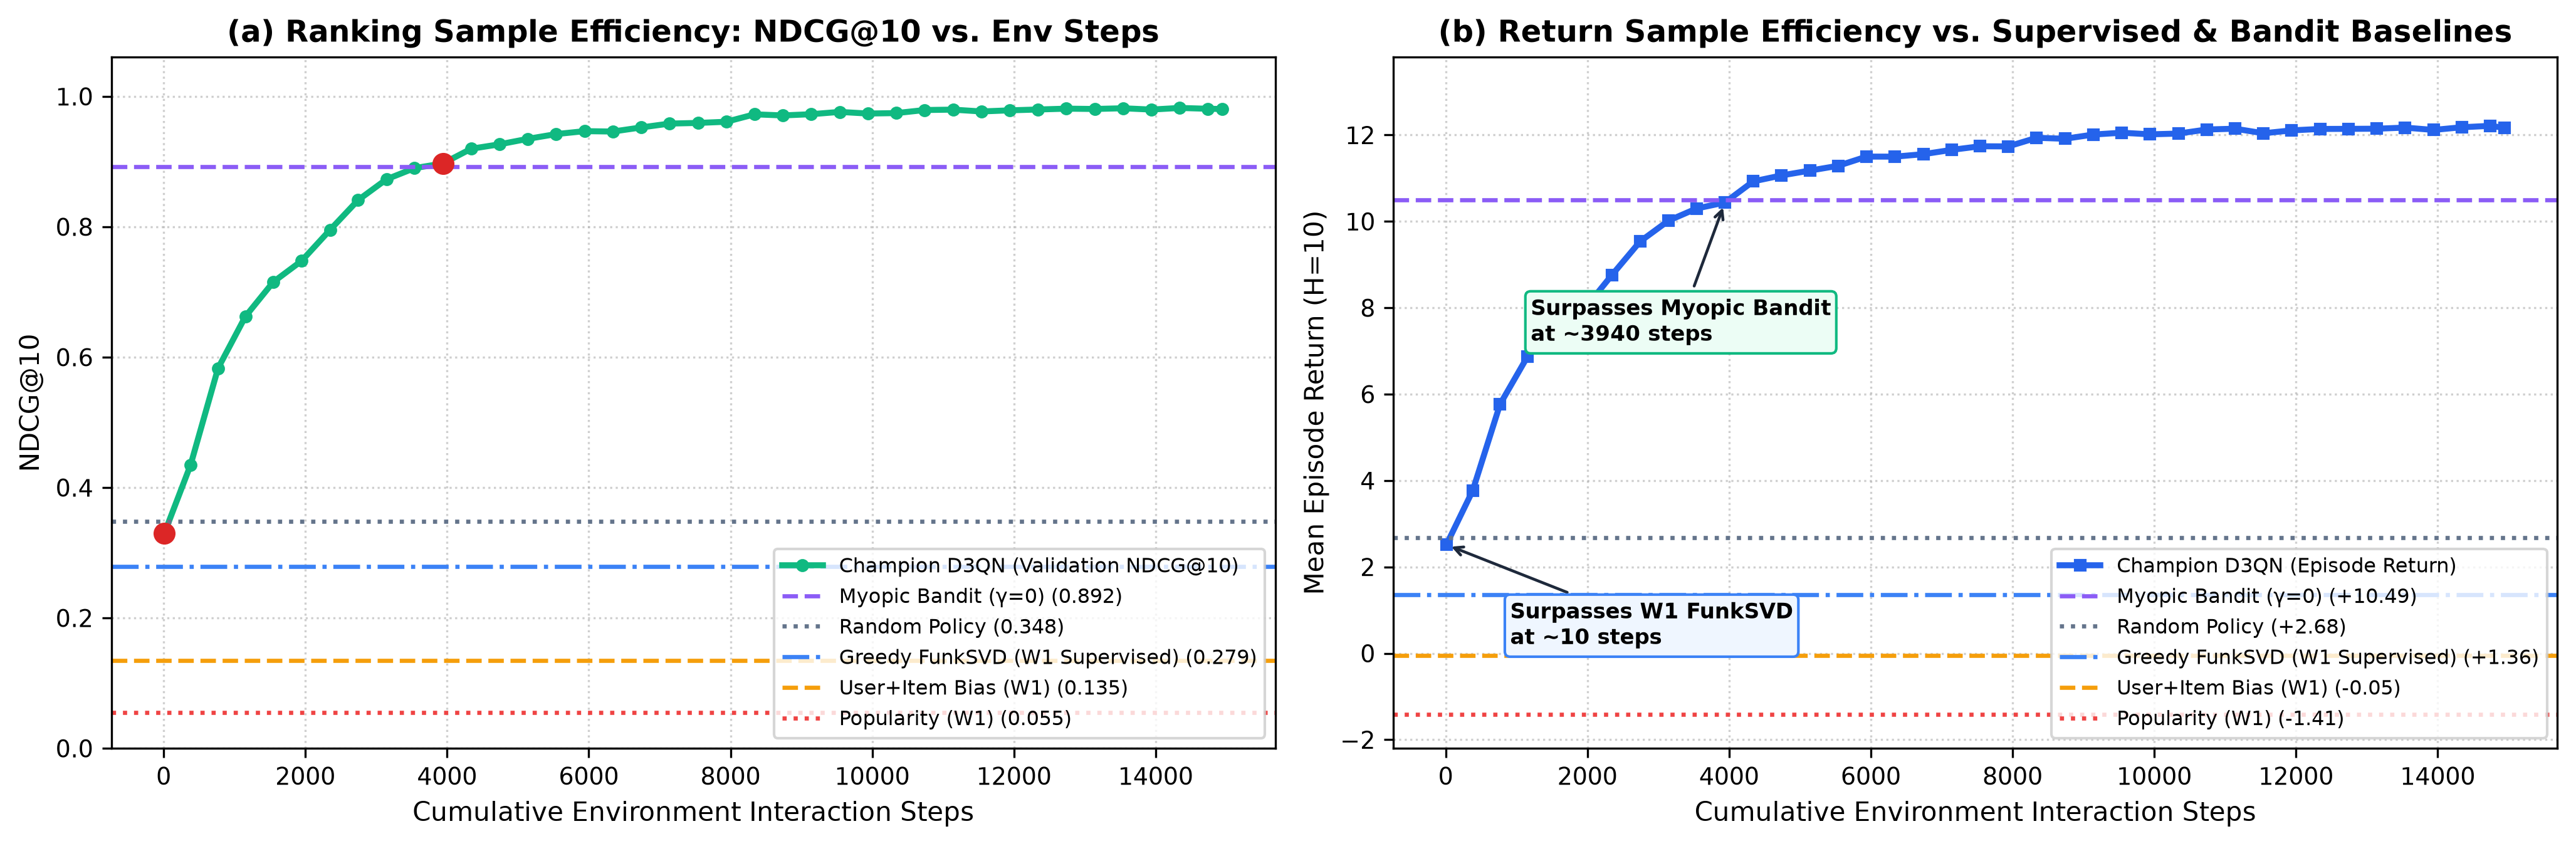
\includegraphics[width=0.96\textwidth]{figures/fig7_sample_efficiency.png}
    \caption{Sample efficiency of the champion D3QN agent as a function of cumulative environment interaction steps across 1,500 training episodes ($14,940$ total steps), compared against Workshop~1/3 static supervised baselines (\texttt{Popularity}, \texttt{BiasOnly}, \texttt{GreedyFunkSVD}), \texttt{Random}, and the \texttt{MyopicBandit} ($\gamma=0$) baseline: (a)~Ranking sample efficiency measured by validation $\text{NDCG@10}$; (b)~Cumulative return sample efficiency measured by mean episode return ($H=10$).}
    \label{fig:sample_efficiency}
\end{figure*}

A central question in sequential recommendation is how many interactive environment transitions a reinforcement learning agent requires to surpass static supervised models trained on massive offline logs. Figure~\ref{fig:sample_efficiency} plots the validation ranking quality ($\text{NDCG@10}$, Panel~a) and mean episode return ($G_{10}$, Panel~b) of the champion D3QN agent every 40 episodes ($\approx 390$--$400$ environment steps) from initialization ($0$~steps) to final convergence ($14,940$~steps across $1,500$~episodes).

\subsubsection{Interaction Milestones to Surpass Baselines}
Tracing the learning trajectory in Figure~\ref{fig:sample_efficiency} reveals three distinct sample-efficiency milestones:
\begin{enumerate}
    \item \textbf{Immediate Dominance Over Heuristic and Static Matrix Factorization Baselines ($\le 381$~Steps / $40$~Episodes):} Even at episode~0 ($\approx 10$ environment steps, prior to replay buffer warmup), the candidate feature projection layer ($\phi(s_t, a)$) provides sufficient inductive structure to achieve $\text{NDCG@10} = 0.3298$ and a mean return of $+2.5138$, already outperforming static \texttt{GreedyFunkSVD} ($\text{NDCG@10} = 0.2785$, Return $= +1.3609$), \texttt{BiasOnly} ($\text{NDCG@10} = 0.1345$, Return $= -0.0451$), and \texttt{Popularity} ($\text{NDCG@10} = 0.0551$, Return $= -1.4121$). By the first logged training checkpoint at \textbf{$381$~environment steps} ($40$~episodes), D3QN reaches $\text{NDCG@10} = 0.4350$, $\text{Precision@10} = 0.4300$, $\text{HR@10} = 0.9700$, and a mean episode return of $+3.7662$ (mean episode length $9.73$ steps), decisively surpassing the \texttt{Random} policy ($\text{NDCG@10} = 0.3480$, Return $= +2.6805$) and all Workshop~1 static baselines.
    \item \textbf{Rapid Climb and Full Session Survival ($768$--$3,144$~Steps / $80$--$320$~Episodes):} By $768$~steps ($80$~episodes), D3QN achieves $\text{NDCG@10} = 0.5831$, $\text{Return} = +5.7700$, and $\text{HR@10} = 1.0000$. By $2,744$~steps ($280$~episodes), the mean episode length reaches the full horizon of $10.00$ steps (zero early session abandonments), with $\text{NDCG@10} = 0.8409$ and $\text{Return} = +9.5358$, passing the $+10.0$ return mark at $3,144$~steps ($\text{Return} = +10.0168$, $\text{NDCG@10} = 0.8728$).
    \item \textbf{Surpassing the Myopic Contextual Bandit ($3,940$--$4,340$~Steps / $400$--$440$~Episodes):} The strongest non-MDP baseline is the neural \texttt{MyopicBandit} ($\gamma=0$), which achieves $\text{NDCG@10} = 0.8924$ and $\text{Return} = +10.4924$. As marked by the red crossover indicator in Figure~\ref{fig:sample_efficiency}(a), D3QN surpasses \texttt{MyopicBandit} in ranking quality at \textbf{$3,940$~environment steps} ($400$~episodes), reaching $\text{NDCG@10} = 0.8971$ ($\text{MAP@10} = 0.8276$, $\text{Return} = +10.4368$). By the next checkpoint at \textbf{$4,340$~environment steps} ($440$~episodes), D3QN surpasses \texttt{MyopicBandit} across both return and ranking criteria simultaneously, achieving $\text{Return} = +10.9268$, $\text{NDCG@10} = 0.9197$, and $\text{Precision@10} = 0.8980$. Thereafter, multi-step Bellman backups continue to refine the policy to a peak validation return of $+12.2125$ at $14,740$~steps ($1,480$~episodes) and final convergence at \textbf{$14,940$~steps} ($1,500$~episodes, wall-clock training time $53.02$~s), yielding test-set $\text{NDCG@10} = 0.9818$ and $\text{Return} = +12.3674$.
\end{enumerate}

\subsubsection{Fair Accounting of the Total Data Budget}
A rigorous comparison between supervised learning (Workshop~1) and reinforcement learning (Workshop~3) requires accounting for both offline representation learning and online policy optimization. In Workshop~1, matrix factorization (FunkSVD) was trained via stochastic gradient descent over $1,895,184$ chronological training ratings across 15 epochs ($\approx 2.84 \times 10^7$ scalar rating updates) to estimate static user and item embeddings ($\mathbf{p}_u, \mathbf{q}_i \in \mathbb{R}^{20}$) and baseline biases ($b_u, b_i$). However, when deployed directly as a sequential recommender (\texttt{GreedyFunkSVD}), those $2.84 \times 10^7$ supervised updates yield only $\text{NDCG@10} = 0.2785$ and $\text{Return} = +1.3609$ because static point-wise error minimization ($\text{RMSE} = 0.8128$) does not optimize sequential slate selection, novelty bonuses, or session survival.

Workshop~3 does not discard the supervised training budget; rather, it leverages the leak-free Workshop~1 latent factors as a compact, pre-trained perceptual representation and adds a lightweight sequential decision layer on top. Requiring only $3,940$--$4,340$ interactive steps to beat a myopic bandit and $14,940$ steps in total---fewer than $0.8\%$ of the $1.895 \times 10^6$ ratings used in Workshop~1---demonstrates that decoupling representation learning (offline matrix factorization) from sequential policy optimization (online D3QN) yields exceptional sample efficiency.

\subsection{Discussion: Strengths, Exploration Trade-offs, and Limitations}
\label{subsec:discussion_limitations}

\subsubsection{Why RL Outperformed Static Supervised Models and Myopic Bandits}
The substantial performance gap between D3QN ($\text{NDCG@10} = 0.9818$, $\text{Return} = +12.3674$) and static \texttt{GreedyFunkSVD} ($\text{NDCG@10} = 0.2785$, $\text{Return} = +1.3609$) stems from three structural properties of interactive recommendation environments:
\begin{itemize}
    \item \textbf{Vulnerability of Static Ranking to Candidate Slate Composition and Early Abandonment:} In our environment, each session presents a stratified candidate pool of $M=50$ items combining top FunkSVD predictions, popular items, and long-tail/decoy items. \texttt{Popularity} ($\text{NDCG@10} = 0.0551$, $\text{Return} = -1.4121$) repeatedly selects globally popular blockbusters that fail to match individual niche tastes, triggering the 5-strike abandonment rule and truncating episodes to a mean length of $5.87$ steps at $K=10$ ($6.01$ steps at $K=20$). \texttt{GreedyFunkSVD} ranks candidates solely by $\hat{r}_{u,i} = \mu + b_u + b_i + \mathbf{p}_u^\top \mathbf{q}_i$, ignoring item self-information novelty, intra-session cosine diversity, and recent negative feedback, resulting in premature termination (mean length $8.50$ steps at $K=10$ and $11.72$ steps at $K=20$).
    \item \textbf{Value of Multi-Step Lookahead ($\gamma = 0.95$ vs.\ $\gamma = 0$):} While \texttt{MyopicBandit} ($\gamma=0$) observes the same 250-dimensional state vector across all 50 candidate slots as D3QN, it maximizes only immediate single-step expected reward $\mathbb{E}[r_t \mid s_t, a_t]$. Consequently, \texttt{MyopicBandit} greedily consumes moderate-novelty hits early in the session, shifting the running belief vector $\bar{\mathbf{q}}_t$ into regions of the candidate slate that deplete high-value compatible items for later steps. At $K=10$, D3QN's multi-step Bellman horizon ($\gamma=0.95$) increases step hit rate from $87.08\%$ to $97.92\%$, $\text{MAP@10}$ from $0.8253$ to $0.9692$, and mean novelty from $14.94$ to $17.96$~bits ($+12.3674$ vs.\ $+10.4924$ return). The advantage of long-horizon planning is amplified even further in extended sessions ($K=20$): \texttt{MyopicBandit} suffers occasional late-session terminations (mean length $19.52$ steps, $\text{Precision@20} = 0.7262$, $\text{NDCG@20} = 0.8068$, $\text{Return} = +16.5601$), whereas D3QN sustains a full $20.00$-step horizon across all 250 test users, achieving $\text{Precision@20} = 0.8398$, $\text{Recall@20} = 0.8849$, $\text{NDCG@20} = 0.9167$, and $\text{Return} = +20.1006$.
\end{itemize}

\subsubsection{Overcoming Popularity Bias vs.\ Intra-List Cohesion}
A major failure mode identified in Workshop~1 was severe popularity bias: global static FunkSVD concentrated recommendations on a narrow subset of mainstream titles, yielding only $8.00\%$ catalog coverage and $9.83$~bits of novelty (while a static baseline recommender reached $14.06$~bits). By explicitly incorporating self-information novelty $I(i) = -\log_2 P(i)$ into the MDP reward and candidate feature vector, D3QN expands catalog coverage by more than $4.5\times$ at $K=10$ to \textbf{$36.64\%$} (and to \textbf{$60.35\%$} at $K=20$), while boosting mean novelty to \textbf{$17.96$~bits} at $K=10$ ($17.27$~bits at $K=20$). Thus, across the test population, D3QN surfaces a wide variety of niche and contemporary long-tail films.

At the same time, an objective inspection of the test-set evaluation results (Section~\ref{sec:results}) reveals an important trade-off between \textit{inter-user catalog coverage} and \textit{intra-list cosine diversity} ($\text{ILD}$). At $K=10$, D3QN exhibits a lower intra-list cosine distance ($\text{ILD} = 0.2731$, rising to $0.4698$ at $K=20$) compared to \texttt{MyopicBandit} ($0.4215$ at $K=10$, $0.6061$ at $K=20$), \texttt{GreedyFunkSVD} ($0.8653$), and unguided \texttt{Random} selection ($0.9664$). This phenomenon has a clear geometric explanation: to guarantee a $97.92\%$ positive hit rate and avoid the $-0.50$ dislike penalty, the D3QN policy learns to select long-tail candidates whose latent vectors $\mathbf{q}_i$ lie within a tight cosine cone around the user's static embedding $\mathbf{p}_u$ and evolving session preference direction $\bar{\mathbf{q}}_t$. While the reward function includes an intra-session diversity bonus ($+0.10(1 - \cos(\mathbf{q}_i, \bar{\mathbf{q}}_t))$), its weight is intentionally subordinate to the primary rating relevance signal ($\pm 1.0$) and novelty bonus ($+0.30\,\tilde{I}(i)$). Consequently, D3QN achieves high inter-user personalization and long-tail discovery across the catalog while maintaining thematically coherent, preference-aligned slates within each individual user session.

\subsubsection{Limitations and Threats to Validity}
To ensure scientific rigor, we highlight three methodological limitations of our study:
\begin{enumerate}
    \item \textbf{Offline Simulator and Preference Oracle Bias:} Because the MovieLens~32M rating matrix exhibits $99.81\%$ sparsity, an interactive RL agent inevitably queries $(u, i)$ pairs that were never observed in the historical logs. Our hybrid environment prioritizes exact held-out ground-truth ratings whenever available and falls back to the leak-free FunkSVD latent preference model ($\hat{r}_{u,i}$ with calibrated Gaussian noise and popularity-penalized specificity) for unobserved pairs. While this follows standard practice in RL-for-RS benchmarks, the agent's learned policy partially exploits the geometry of the FunkSVD embedding space; deploying the policy in live production A/B tests could exhibit a reality gap where user preferences deviate from bilinear factor inner products.
    \item \textbf{Discrete Candidate Pre-Selection ($M=50$):} Evaluating Q-values over all $11,589$ active catalog movies at every step would incur high computational overhead and severe action-space variance. Constraining the action space to a stratified slate of $M=50$ candidates per episode makes D3QN training highly tractable ($53.02$~s on a single GPU), but bounds the policy's recall ceiling by the quality of the first-stage candidate generator.
    \item \textbf{Temporal Cold-Start Vulnerability:} As quantified in Workshop~1, $90.06\%$ of raw chronological test interactions in MovieLens~32M involve newly arrived users or newly released items absent from the training window. Because our state representation $s_t$ relies on pre-trained user factors $\mathbf{p}_u \in \mathbb{R}^{20}$ at $t=1$, strictly cold-start users ($\mathbf{p}_u = \mathbf{0}$) begin with an uninformative prior until several interactive steps populate the dynamic belief centroid $\bar{\mathbf{q}}_t$.
\end{enumerate}

\section{Conclusions and Future Work}
\label{sec:conclusions}

This work formulated sequential movie recommendation on the MovieLens~32M dataset as a finite-horizon Markov Decision Process and designed a Dueling Double Deep Q-Network (D3QN) to optimize long-term user satisfaction, catalog discovery, and session retention. Building strictly on the leak-free chronological data splits and 20-dimensional FunkSVD latent representations established in Workshop~1, we constructed a 250-dimensional sequential state space that tracks dynamic session-item cosine similarities, static FunkSVD predictions, self-information novelty, visited-action masks, user/session latent embeddings, and session progress indicators across a stratified $M=50$ action space.

Comprehensive empirical evaluations across nine hyperparameter configurations and six baseline policies at horizons $K=10$ and $K=20$ support four principal conclusions:
\begin{enumerate}
    \item \textbf{Superior Sequential Ranking and Return:} The tuned D3QN champion ($\text{lr}=5\times 10^{-4}$, $\gamma=0.95$, $\epsilon_{\text{decay}}=0.995$, L2 $= 10^{-5}$) achieves a test-set episode return of $+12.3674$, $\text{Precision@10} = 0.9792$, $\text{NDCG@10} = 0.9818$, $\text{MAP@10} = 0.9692$, and $\text{HR@10} = 1.0000$ at $K=10$, and scales robustly to $K=20$ with a return of $+20.1006$ and $\text{NDCG@20} = 0.9167$.
    \item \textbf{Value of Multi-Step Planning Over Myopic Bandits and Static Rankers:} D3QN outperforms Workshop~1 static FunkSVD ($\text{NDCG@10} = 0.2460$) and sequential \texttt{GreedyFunkSVD} ($\text{NDCG@10} = 0.2785$, Return $= +1.3609$) by over $+0.70$ in $\text{NDCG@10}$, and surpasses a matched neural \texttt{MyopicBandit} ($\gamma=0$, $\text{NDCG@10} = 0.8924$, Return $= +10.4924$) by $+17.9\%$ in cumulative return at $K=10$ and $+21.4\%$ at $K=20$, confirming that non-myopic Bellman backups ($\gamma=0.95$) preserve slate quality and prevent premature session abandonment.
    \item \textbf{Mitigation of Popularity Bias:} By integrating self-information novelty into the sequential reward structure, D3QN expands catalog coverage from Workshop~1's $8.00\%$ to $36.64\%$ at $K=10$ and $60.35\%$ at $K=20$, while elevating mean recommendation novelty from $9.83$~bits to $17.96$~bits.
    \item \textbf{High Sample Efficiency:} Leveraging pretrained matrix factorization embeddings, D3QN surpasses all static supervised baselines within $381$ environment interaction steps ($40$ episodes) and overtakes the myopic contextual bandit within $3,940$--$4,340$ steps ($400$--$440$ episodes), converging in $14,940$ steps ($53.02$~s).
\end{enumerate}

\textbf{Future Work:} Several promising directions grounded in advanced policy optimization and multi-agent reinforcement learning~\cite{sierra2026rl} extend this research toward industrial-scale deployment. First, replacing discrete $M=50$ value-based selection with \textit{policy-based Actor-Critic architectures}---guided by the Policy Gradient Theorem $\nabla_\theta J(\theta) = \mathbb{E}_{\pi_\theta}[\nabla_\theta \log \pi_\theta(a \mid s) Q^{\pi_\theta}(s, a)]$ and critic TD advantage estimation $\delta_t = r_{t+1} + \gamma V_\phi(s_{t+1}) - V_\phi(s_t)$, such as Trust Region Policy Optimization (TRPO, $\bar{D}_{\text{KL}}(\theta_{\text{old}}, \theta) \le \delta$) or Proximal Policy Optimization (PPO, $L^{\text{CLIP}}(\theta) = \mathbb{E}[\min(r_t(\theta)\hat{A}_t, \text{clip}(r_t(\theta), 1-\epsilon, 1+\epsilon)\hat{A}_t)]$)~\cite{sierra2026rl} outputting a continuous prototype action vector $\mathbf{a}_t \in \mathbb{R}^{20}$ coupled with Approximate Nearest Neighbor (FAISS) retrieval---would enable direct policy optimization over the full catalog of $80,000+$ titles. Second, modeling multi-stakeholder recommendation (balancing user satisfaction, content provider fairness, and platform revenue) as a cooperative-competitive Multi-Agent RL system under the Centralized Training with Decentralized Execution (CTDE) paradigm~\cite{sierra2026rl}, alongside Conservative Q-Learning (CQL) and hybrid content-collaborative GNN encoders, will allow sequential policies to generalize across both multi-objective constraints and the $90.06\%$ cold-start regime.


\bibliographystyle{IEEEtran}
\bibliography{bibliography}

\end{document}
